%% Elsevier single-column submission format for Digital Chemical Engineering
\documentclass[a4paper,fleqn]{cas-sc}

\usepackage[authoryear,longnamesfirst]{natbib}
\usepackage{amsmath}
\usepackage{amssymb}
\usepackage{capt-of}
\usepackage{xcolor}
\usepackage{float}
\usepackage{mdframed}
\usepackage{needspace}
\usepackage{lineno}
\graphicspath{{./}{docs/DCHE-D-26-00020/}}

\definecolor{revDefault}{RGB}{0,0,255}
\definecolor{revRoneTen}{RGB}{0,116,153}
\definecolor{revRoneSixteen}{RGB}{217,95,2}
\definecolor{revRoneTwentyFive}{RGB}{0,140,72}
\definecolor{revRoneTwentySeven}{RGB}{140,81,10}
\definecolor{revRtwoOne}{RGB}{171,71,188}
\definecolor{revRtwoTwo}{RGB}{196,30,58}
\definecolor{revRtwoFour}{RGB}{46,125,50}
\definecolor{revRtwoFive}{RGB}{94,53,177}

\newcommand{\rev}[1]{#1}
\newcommand{\revitem}[2]{#2}
\newenvironment{revblock}{}{}
\newenvironment{revblockr110}{}{}
\newenvironment{revblockr116}{}{}
\newenvironment{revblockr125}{}{}
\newenvironment{revblockr127}{}{}
\newenvironment{revblockr21}{}{}
\newenvironment{revblockr22}{}{}
\newenvironment{revblockr24}{}{}
\newenvironment{revblockr25}{}{}

\newenvironment{figrev}{}{}
\newenvironment{figrevr125}{}{}
\newenvironment{figrevr21}{}{}
\newenvironment{figrevr25}{}{}

%%% Author macros
\def\tsc#1{\csdef{#1}{\textsc{\lowercase{#1}}\xspace}}
\tsc{WGM}
\tsc{QE}

\ExplSyntaxOn
\keys_set:nn { stm / mktitle } { nologo }
\cs_set:Npn \__first_footerline:
{
    \group_begin:
    \small
    \sffamily
    \ifnum\theblind>0\relax
    \else
        \__short_authors:
    \fi
    \group_end:
}
\ExplSyntaxOff

\begin{document}
\let\WriteBookmarks\relax
\def\floatpagepagefraction{1}
\def\textpagefraction{.001}

\shorttitle{An Interpretable Statistical Surrogate of Activated Sludge Systems}
\shortauthors{}

\title[mode=title]{\rev{An Interpretable Statistical Surrogate of Activated Sludge Systems that Preserves Mass Conservation and Component Non-Negativity}}

\author{}

\begin{abstract}
\rev{Standard machine-learning surrogates of activated sludge systems can predict effluent composites accurately, yet their component-space predictions need not satisfy exact stoichiometric mass conservation or componentwise non-negativity. This article develops Invariant-Constrained Second-Order Regression (ICSOR), an interpretable surrogate that enforces both requirements within a single steady-state formulation through a partitioned second-order feature map, a learned cross-component coupling matrix, deterministic recursive coupled-QP estimation, and a hierarchical deployment rule combining a closed-form affine invariant projection with a linear program. On a 10,000-sample ASM2d-TSN continuous stirred tank reactor benchmark, ICSOR was compared against nine unconstrained baselines spanning gradient-boosted trees (XGBoost, LightGBM, CatBoost), other ensembles (Random Forest, AdaBoost), Support Vector Regression, $k$-Nearest Neighbors, Partial Least Squares, and a multilayer perceptron. ICSOR was the only model that produced no mass-conservation violations and no non-negativity violations on the test set, whereas every unconstrained baseline violated conservation on all test samples. Despite operating under these physical constraints, ICSOR maintained competitive aggregate accuracy in the reported composite space, attained the lowest normalized area under the RMSE learning curve across the full dataset-size sweep, and exhibited the smallest train-validation RMSE gap among the competitively accurate models.}
\end{abstract}

\begin{graphicalabstract}
\centering
\begin{figrev}
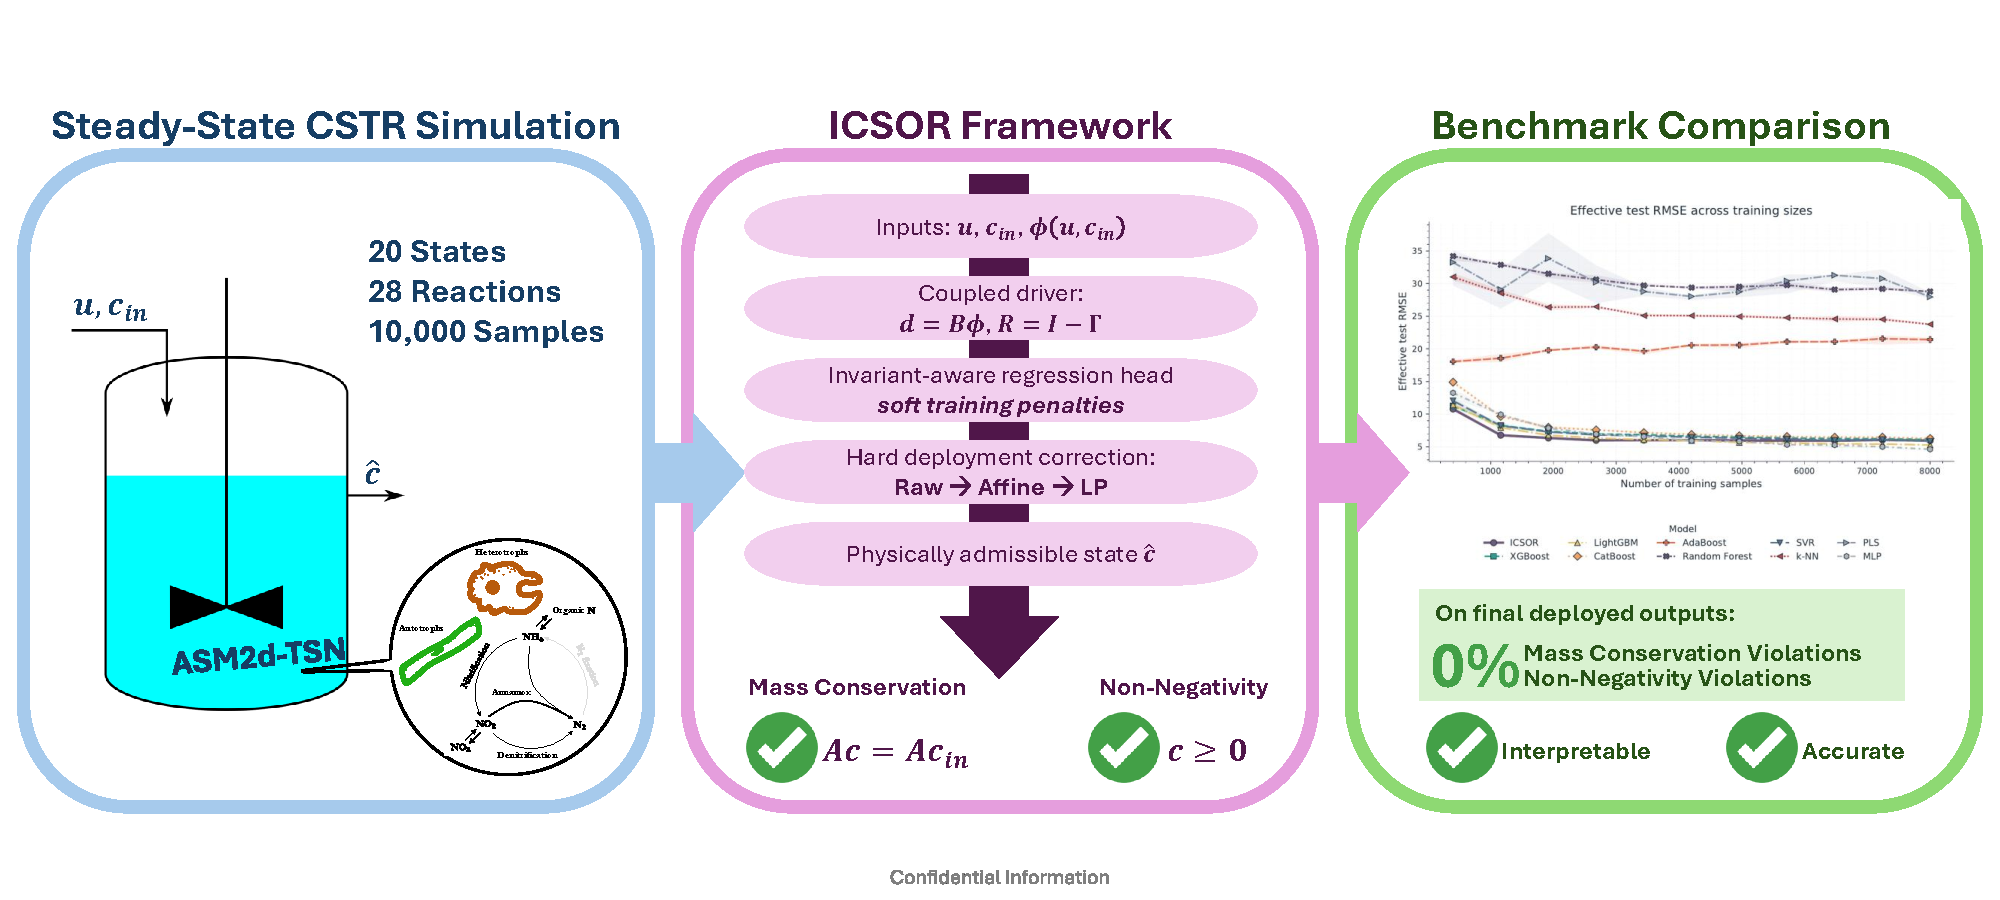
\includegraphics[width=0.98\linewidth]{graphical_abstract}
\end{figrev}
\end{graphicalabstract}

\begin{highlights}
\item \rev{ICSOR enforces exact mass conservation and non-negativity in one surrogate.}
\item \rev{Only model with zero conservation and non-negativity violations on all test samples.}
\item \rev{Lowest mean held-out RMSE at the smallest retained dataset size among all ten models.}
\item \rev{Lowest normalized area under the RMSE learning curve across dataset sizes.}
\item \rev{Smallest train-validation RMSE gap among competitively accurate surrogate models.}
\end{highlights}

\begin{keywords}
\rev{Wastewater treatment \sep Activated sludge model \sep Physics-informed machine learning \sep Surrogate modeling \sep Constrained optimization \sep Stoichiometric mass conservation \sep Interpretable regression}
\end{keywords}

\maketitle

\section*{\revitem{revRoneTen}{Nomenclature}}
\begin{revblockr110}
\begin{tabbing}
\hspace{2.5cm} \= \kill
$A$ \> Full-row-rank invariant matrix defining the null space of the stoichiometric matrix \\
$b$ \> Baseline forcing vector of the blockwise driver ($b \in \mathbb{R}^{F}$) \\
$B$ \> Second-order driver coefficient matrix \\
$c_{aff}$ \> Affine invariant projection of the raw coupled state onto the conservation manifold \\
$c_{in}$ \> Influent ASM component concentration vector ($c_{in} \in \mathbb{R}^{F}$) \\
$c_{out}$ \> True steady-state effluent ASM component concentration vector ($c_{out} \in \mathbb{R}^{F}$) \\
$c_{raw}$ \> Unconstrained coupled component prediction before affine presolve \\
$\hat{c}$ \> Final deployed ICSOR ASM component prediction \\
$\widehat{C}$ \> Fitted non-negative component prediction matrix used in training \\
$D$ \> Total dimension of the second-order feature map \\
$F$ \> Number of mechanistic ASM components \\
$\mathcal{G}$ \> Admissible set for $\Gamma$ (zero diagonal, box bounds, conditioning threshold) \\
$\Gamma$ \> Learned ASM component coupling matrix \\
$I_{comp}$ \> Composition matrix mapping ASM components to measured composites ($I_{comp} \in \mathbb{R}^{K \times F}$) \\
$K$ \> Number of measured composite variables \\
$\kappa(\cdot)$ \> Matrix condition number \\
$\lambda_B$ \> Ridge regularization weight on $B$ \\
$\lambda_\Gamma$ \> Ridge regularization weight on $\Gamma$ \\
$\lambda_{inv}$ \> Invariant-residual penalty weight in the training objective \\
$\lambda_{sys}$ \> Coupled-system consistency penalty weight in the training objective \\
$M_{op}$ \> Number of operational variables \\
$N$ \> Number of steady-state training samples \\
$N_{rxn}$ \> Number of reactions in the mechanistic model \\
$R$ \> Coupled-system matrix, $R = I_F - \Gamma$ \\
$u$ \> Operational input vector ($u \in \mathbb{R}^{M_{op}}$) \\
$w_c$ \> Componentwise weight vector used in deployed correction \\
$y_{ext}$ \> Reported measured effluent composite vector ($y_{ext} \in \mathbb{R}^{K}$) \\
$\hat{y}_{ext}$ \> Reported composite prediction, $\hat{y}_{ext} = I_{comp}\hat{c}$ \\
$\nu$ \> Stoichiometric matrix ($\nu \in \mathbb{R}^{N_{rxn} \times F}$) \\
$\xi$ \> Net reaction progress vector \\
$\Phi$ \> Feature matrix collecting $\phi$ row-wise over the training set ($\Phi \in \mathbb{R}^{N \times D}$) \\
$\phi$ \> Partitioned second-order feature map \\
$\Theta_{cc}$ \> Influent--influent second-order driver block ($\Theta_{cc} \in \mathbb{R}^{F \times F^2}$) \\
$\Theta_{uc}$ \> Operating--influent interaction driver block ($\Theta_{uc} \in \mathbb{R}^{F \times (M_{op}F)}$) \\
$\Theta_{uu}$ \> Operating--operating second-order driver block ($\Theta_{uu} \in \mathbb{R}^{F \times M_{op}^2}$) \\
$W_{in}$ \> First-order influent driver block ($W_{in} \in \mathbb{R}^{F \times F}$) \\
$W_u$ \> First-order operating driver block ($W_u \in \mathbb{R}^{F \times M_{op}}$) \\
$\otimes$ \> Kronecker product \\
\end{tabbing}
\end{revblockr110}

\section{Introduction}

Water pollution presents a critical environmental and public health challenge worldwide, with particularly severe repercussions in developing nations (Lin et al., 2022; Madhav et al., 2020). Biological wastewater treatment systems, particularly those based on the activated sludge process, are the dominant approach applied to combat this issue (Duan et al., 2022). However, their modeling and analysis present formidable engineering and computational challenges (Xiao et al., 2025). The underlying biophysical mechanisms are governed by the Activated Sludge Models (ASM) (Henze et al., 2006), which rely on coupled, multiplicative non-linear kinetic expressions to describe microbial growth and substrate consumption. This inherent non-linearity limits the practical application of transparent analytical methods for process design, frequently forcing engineers to rely on iterative trial-and-error approaches or computationally expensive heuristic algorithms (Aboagye et al., 2021; Padron-Paez et al., 2020).

In response to the computational and mathematical complexity inherent in non-linear Activated Sludge Models, research has increasingly focused on developing surrogate models to approximate the behavior of biological wastewater treatment systems (Bhosekar \& Ierapetritou, 2018; Durkin et al., 2024; Tsochatzidi et al., 2025). Traditional approaches have explored linearization techniques (Li et al., 2020; Yang et al., 2014) and multivariable polynomial fitting (Ahn et al., 2014; Kim et al., 2009; Lim et al., 2011). While linear methods like Partial Least Squares (PLS) offer interpretable mappings, they inherently struggle to capture the severe non-linearities of microbial kinetics without extensive feature engineering; indeed, comparative wastewater studies report substantial error reductions when linear PLS is replaced by kernel-based or nonlinear inner-model variants (Liu et al., 2021; Woo et al., 2009; Yang et al., 2021). To overcome these limitations, the machine learning (ML) paradigm has emerged as a powerful route for approximating highly non-linear wastewater-treatment behavior (Croll et al., 2023; Nazlabadi et al., 2021). Recent wastewater evidence further shows that, when predictive accuracy alone is the criterion, modern ML models can outperform mechanistic ASM baselines for effluent nitrogen prediction (Wang et al., 2025). A wide array of data-driven algorithms---ranging from distance-based methods like k-Nearest Neighbors (k-NN) and PLS (Khatri et al., 2020; Wold et al., 2001), to kernel methods like Support Vector Regression (SVR) (Fang et al., 2011), tree-based ensembles such as Random Forest (RF), AdaBoost, XGBoost, LightGBM, and CatBoost (Sadri Moghaddam \& Mesghali, 2023; Wang et al., 2025; Yang et al., 2025), and Artificial Neural Networks (ANN) (Asadi et al., 2017; Bagherzadeh et al., 2021; Mao et al., 2024)---have demonstrated strong predictive capabilities for effluent quality. 

\begin{revblock}
Despite their predictive accuracy, these standard ML algorithms remain structurally blind to a central physical requirement of activated sludge systems: material cannot be created or destroyed arbitrarily across the modeled control volume. A surrogate may fit observed effluent behavior well while still implying an impossible redistribution of the underlying ASM components, thereby violating the mass balances that govern COD, nitrogen, or phosphorus transfer. Related composition-preserving ML studies show that even accurate tree-based predictors can exhibit persistent unphysical conservation residuals unless an explicit corrective mechanism is imposed (Sturm \& Silva, 2025). At the same time, physically admissible concentration states must remain componentwise non-negative. These two requirements are inseparable in practice. A surrogate that conserves mass but predicts negative concentrations is still unusable, and a surrogate that preserves non-negativity while violating mass conservation remains physically misleading.

Recent scientific-ML literature shows that satisfying both requirements simultaneously is nontrivial. A substantial class of methods enforces conservation alone through conservative flux formulations, stoichiometric architectures, projection operators, Bayesian reconciliation, or completion strategies, but does not guarantee non-negativity of the corrected state (Beucler et al., 2021; Geiss et al., 2022; Hansen et al., 2024; Harder et al., 2022; Sturm \& Silva, 2025; Sturm \& Wexler, 2020, 2022). In that broader literature, completion methods reconstruct withheld variables to satisfy linear equality constraints (Beucler et al., 2021), Bayesian reconciliation treats conservation as a probabilistic update (Hansen et al., 2024), and recent atmospheric-composition studies use stoichiometric null-space constructions and invariant-restoring nudges to keep learned states on the conservation manifold (Sturm \& Silva, 2025; Sturm \& Wexler, 2020, 2022). Closely related soft-constraint approaches, such as physics-informed neural networks, can encourage physically plausible behavior but generally provide neither exact conservation nor strict positivity guarantees; more generally, soft-penalty conservation treatments need not drive residual violations to zero at deployment (Hansen et al., 2024; Raissi et al., 2019). Positivity-only output transformations---whether activation-function clipping, ReLU output layers, or manual thresholding---can prevent negative states, but without an accompanying conservation mechanism they do not by themselves enforce global material balance (Kircher \& Votsmeier, 2025; Ruckstuhl et al., 2021; Utkarsh et al., 2025). Conversely, conservative projection steps that ignore positivity can still generate infeasible negative states in practice, which is precisely why joint enforcement remains difficult (Kircher \& Votsmeier, 2025).

A smaller body of work has reported simultaneous enforcement of conservation and non-negativity. Kircher and Votsmeier (2025) develop positivity-preserving conservative corrections for mechanistic kinetics surrogates in atmospheric chemistry and heterogeneous catalysis, while Sturm et al. (2023) show in aerosol transport that mass-preserving scaling can maintain both total conservation and non-negativity for advected aerosol superspecies. Min et al. (2024) and Utkarsh et al. (2025) likewise propose hard-constrained learning frameworks that can impose equality and inequality constraints together in more general machine-learning settings. These results demonstrate that dual physical guarantees are achievable, but they arise in application settings whose state definitions, constraints, and deployment objectives differ substantially from those of activated sludge process surrogates.

This gap is consequential for wastewater engineering. Activated sludge models couple multiple conserved material inventories with biologically and chemically constrained component states, so violations of either mass conservation or non-negativity can distort interpretation, confound process optimization, and undermine confidence in surrogate-assisted design (Hansen et al., 2024; Liu et al., 2021; Straus \& Skogestad, 2018; Tang et al., 2026). A physically constrained data-driven model would therefore offer several practical benefits: it would preserve the bookkeeping needed for COD, nitrogen, and phosphorus analysis, prevent impossible negative component concentrations, reduce reliance on ad hoc clipping or reconciliation (Ba-Alawi et al., 2021; Kircher \& Votsmeier, 2025), and yield predictions that remain more defensible as operating conditions and influent loads vary. Yet, to our knowledge, prior wastewater surrogate and review literature has not reported an activated sludge surrogate that provides hard guarantees of both stoichiometric mass conservation and componentwise non-negativity within a single interpretable steady-state framework (Kircher \& Votsmeier, 2025; Newhart et al., 2019; Wang et al., 2025).

This study addresses that need through the development of Invariant-Constrained Second-Order Regression (ICSOR), a physics-informed surrogate framework for steady-state activated sludge systems. ICSOR is designed to answer a practical question: given a steady-state influent condition and operating point, what effluent state should be predicted if the surrogate is required to remain physically admissible by construction? Rather than treating physical consistency as a soft regularizer or a purely diagnostic afterthought, the framework is built so that deployed predictions satisfy both mass-conservation requirements and non-negativity requirements simultaneously.

To do so, ICSOR couples an interpretable second-order surrogate with a hard physical correction performed in ASM component space. The regression structure retains transparent operating-condition, influent, and interaction effects, while the deployment step removes states that would violate the admissible physical region. The result is a surrogate that remains analytically structured and data-driven, yet is constrained to return only physically meaningful steady-state predictions.

\revitem{revRtwoOne}{This structural design also distinguishes ICSOR from interpretable baselines such as PLS and from post hoc sensitivity analyses applied to black-box models. PLS loading weights describe linear latent directions and are fitted without any physical-admissibility requirement, so they are free to reflect statistically efficient but physically unconstrained projections. ANN sensitivity analyses are local, post hoc response diagnostics that describe how a particular prediction changes with a small input perturbation; they do not expose the global model structure and are computed from a model whose parameters were likewise fitted without conservation or positivity requirements. By contrast, ICSOR separates first-order operating effects, first-order influent effects, within-subspace curvature, cross-subspace interactions, and cross-component redistribution in the predicted ASM state, and every coefficient block is estimated under hard enforcement of stoichiometric mass conservation and componentwise non-negativity. Because the training objective in Eq.~\eqref{eq:training-objective} penalizes invariant mismatch and the deployment step enforces exact conservation and non-negativity, the learned coefficient values are shaped by the requirement that the resulting predictions must lie in the physically admissible region. The coefficients therefore tend to be more physically inclined than those of an unconstrained model, not because a physical prior is imposed on individual parameters, but because the admissible prediction space itself excludes physically impossible redistributions during fitting.}

The objective of this article is to formulate the ICSOR framework as an analytically structured surrogate and to evaluate its efficacy on a standalone Continuous Stirred Tank Reactor (CSTR). By comparing ICSOR against established unconstrained baselines, this study assesses whether the proposed model can achieve competitive predictive accuracy while explicitly guaranteeing the parsimony, interpretability, and rigorous physical consistency required for reliable process analysis. The framework presented herein is strictly bounded to steady-state predictions; while it guarantees mass conservation and non-negativity, it does not claim to enforce full kinetic or thermodynamic feasibility, nor does it replace dynamic trajectory simulators. Instead, it occupies a necessary middle ground: a surrogate simple enough to be estimated transparently from data, yet mathematically constrained to respect the fundamental physical constraints of wastewater engineering.
\end{revblock}

\section{\rev{Theory and Calculation}}
\begin{revblock}

\subsection{Physical Scope, State Spaces, and Notation}

A fixed reactor block or process unit represented by steady-state samples is considered. The system boundary used to define influent and effluent states is identical to the boundary used to define stoichiometric conservation. Any external source or sink that crosses that boundary must therefore be represented in the adopted stoichiometric model; otherwise, it lies outside the present conservation claim.

ICSOR is formulated natively in ASM component space. Its scientific output is the effluent component vector itself, not a measured aggregate. Measured composites are obtained only afterward through an external composition matrix. This choice is deliberate because mass conservation and componentwise non-negativity are both defined in ASM component coordinates.

Let $M_{op}$ be the number of operational variables, $F$ the number of ASM components, $K$ the number of reported composite variables, and $N_{rxn}$ the number of reactions. Single-sample vectors are written as column vectors. The following state spaces and operators are defined:
\begin{itemize}
    \item $u \in \mathbb{R}^{M_{op}}$: Operational input vector (e.g., hydraulic retention time, aeration intensity).
    \item $c_{in} \in \mathbb{R}^{F}$: Influent ASM component concentration vector.
    \item $c_{out} \in \mathbb{R}^{F}$: True steady-state effluent ASM component concentration vector.
    \item $\hat{c} \in \mathbb{R}^{F}$: Final deployed ICSOR component prediction.
    \item $y_{ext} \in \mathbb{R}^{K}$: Reported measured composite vector.
    \item $I_{comp} \in \mathbb{R}^{K \times F}$: Composition matrix mapping ASM component concentrations to reported composites, such that $y_{ext} = I_{comp}c_{out}$.
    \item $\nu \in \mathbb{R}^{N_{rxn} \times F}$: Stoichiometric matrix.
\end{itemize}

The linear composition map $I_{comp}$ remains external to the model itself. In the common wastewater-reporting case where its rows are entrywise non-negative, non-negative component predictions imply non-negative reported composites automatically. Thus ICSOR places the hard non-negativity guarantee where it is physically meaningful, namely on the predicted ASM component state.

\begin{revblockr22}
\subsection{Stoichiometric Structure and Conserved Quantities}

Let $\nu \in \mathbb{R}^{N_{rxn} \times F}$ be the stoichiometric matrix written in the adopted ASM component basis. For a steady-state sample, define the net reaction progress vector $\xi \in \mathbb{R}^{N_{rxn}}$, scaled into concentration-equivalent units, such that the net change across the control volume is:
\begin{equation}
\label{eq:stoichiometric-change}
 c_{out} - c_{in} = \nu^T \xi
\end{equation}
The vector $\xi$ is rarely observed directly. To eliminate it and isolate the conserved quantities, a full-row-rank matrix $A \in \mathbb{R}^{q \times F}$ is introduced whose rows span the left null space of $\nu$, so that $A\nu^T = 0$. Multiplying the stoichiometric change relation by $A$ yields:
\begin{equation}
\label{eq:invariant-conservation}
 A(c_{out} - c_{in}) = A \nu^T \xi = 0 \quad \implies \quad A c_{out} = A c_{in}
\end{equation}
This invariant-matrix construction follows the same mathematical idea used by Sturm and Wexler (2020) in mass-conserving photochemical surrogates, where a null-space matrix is used to preserve elemental inventories exactly. In the present setting, the conserved rows of $A$ represent wastewater-material inventories implied by the adopted ASM reaction network and system boundary rather than atmospheric atom counts.
Each row of $A$ represents one independent conserved combination of ASM components implied by the adopted reaction network and system boundary. The basis of $A$ is not unique, but once it is fixed, the invariant relation $Ac_{out} = Ac_{in}$ defines the exact conservation law that deployed ICSOR predictions must satisfy.
\end{revblockr22}

\subsection{Coupled Second-Order Driver and Prediction-Space Training}

Operational variables $u$ alter the process environment, whereas influent concentrations $c_{in}$ determine the material inventory presented to that environment (de Araujo et al., 2013; Machado et al., 2014). ICSOR keeps these roles explicit by using a partitioned second-order feature map:
\begin{equation}
\label{eq:feature-map}
\phi(u, c_{in}) = \begin{bmatrix}
1 \\
 u \\
 c_{in} \\
 u \otimes u \\
 c_{in} \otimes c_{in} \\
 u \otimes c_{in}
\end{bmatrix} \in \mathbb{R}^{D}
\end{equation}
where $\otimes$ denotes the Kronecker product under column-wise vectorization and $D = 1 + M_{op} + F + M_{op}^2 + F^2 + M_{op}F$.

The feature map drives a latent component-space forcing vector rather than the final deployed prediction directly:
\begin{equation}
\label{eq:latent-driver}
 r(u, c_{in}) = B \phi(u, c_{in})
\end{equation}
Using a latent driver rather than predicting the deployed state directly is also consistent with stoichiometry-driven flux-to-tendency architectures such as the conservation-law neural-network formulation of Sturm and Wexler (2022). The present article adopts that separation in a different way: ICSOR keeps the driver explicitly linear-quadratic and interpretable, then combines it with a learned coupling matrix and a separate constrained deployment step rather than embedding a fixed stoichiometric layer inside a deep network.

Using the same partitioned basis, the driver can be written blockwise as
\begin{equation}
\label{eq:blockwise-driver}
 r(u, c_{in}) = b + W_u u + W_{in} c_{in} + \Theta_{uu}(u \otimes u) + \Theta_{cc}(c_{in} \otimes c_{in}) + \Theta_{uc}(u \otimes c_{in}),
\end{equation}
with $b \in \mathbb{R}^{F}$, $W_u \in \mathbb{R}^{F \times M_{op}}$, $W_{in} \in \mathbb{R}^{F \times F}$, $\Theta_{uu} \in \mathbb{R}^{F \times M_{op}^2}$, $\Theta_{cc} \in \mathbb{R}^{F \times F^2}$, and $\Theta_{uc} \in \mathbb{R}^{F \times (M_{op}F)}$.

Cross-component dependence is introduced explicitly through a learned coupling matrix $\Gamma \in \mathbb{R}^{F \times F}$. In this study, $\Gamma$ is estimated in an admissible set that fixes its diagonal to zero, bounds its off-diagonal entries, and rejects choices that make $R = I_F - \Gamma$ poorly conditioned. The coupled relation is written as
\begin{equation}
\label{eq:coupled-relation}
 R c = r(u, c_{in}), \qquad R = I_F - \Gamma
\end{equation}

The sign of $B$ is not constrained. That choice is deliberate: increasing and decreasing effects are both allowed in the latent driver, while non-negativity is enforced later where it matters physically, on the predicted component state itself.

Over a dataset of $N$ steady-state samples, let $\Phi \in \mathbb{R}^{N \times D}$ collect the feature rows, let $C_{in} \in \mathbb{R}_{+}^{N \times F}$ collect influent component states, and let $C_{out} \in \mathbb{R}_{+}^{N \times F}$ collect effluent component targets. ICSOR introduces a fitted non-negative component prediction matrix $\widehat{C} \in \mathbb{R}_{+}^{N \times F}$ and estimates $(B, \Gamma, \widehat{C})$ through the coupled objective
\begin{equation}
\label{eq:training-objective}
\begin{aligned}
(\widehat{B}, \widehat{\Gamma}, \widehat{C}) = {}&
\arg\min_{B,\, \Gamma \in \mathcal{G},\, \widehat{C} \in \mathbb{R}_{+}^{N \times F}}
\Bigl\|
C_{out} - \widehat{C}
\Bigr\|_F^2 \\
&+ \lambda_{inv}
\Bigl\|
(\widehat{C} - C_{in})A^T
\Bigr\|_F^2 \\
&+ \lambda_{sys}
\Bigl\|
\widehat{C}(I_F - \Gamma)^T - \Phi B^T
\Bigr\|_F^2 \\
&+ \lambda_B \|B\|_F^2
+ \lambda_\Gamma \|\Gamma\|_F^2.
\end{aligned}
\end{equation}

Each term has a distinct role. The first term fits effluent ASM components directly. The second penalizes invariant mismatch in component space. The third forces consistency between the fitted states and the coupled driver relation. The ridge penalties stabilize the driver and coupling estimates.

\subsection{Deployment-Time Inference with Exact Conservation and Non-Negativity}

Training determines $\widehat{B}$ and $\widehat{\Gamma}$. Deployment then predicts a new component state through a staged inference rule: a direct coupled evaluation, a closed-form affine projection, and, only when non-negativity is still violated, a final linear program. For a new sample $(u_*, c_{in,*})$, define
\begin{equation}
\label{eq:deployment-definitions}
\phi_* = \phi(u_*, c_{in,*}), \qquad d_* = \widehat{B}\phi_*, \qquad \widehat{R} = I_F - \widehat{\Gamma}.
\end{equation}

Whenever $\widehat{R}$ is nonsingular, the unconstrained coupled state is
\begin{equation}
\label{eq:raw-coupled-state}
 c_{raw} = \widehat{R}^{-1} d_*.
\end{equation}

A cheap affine presolve then restores exact invariants without yet enforcing non-negativity. The nearest invariant-consistent state to the raw predictor is
\begin{equation}
\label{eq:affine-presolve}
 c_{aff} = \arg\min_{c \in \mathbb{R}^{F}} \; \|c - c_{raw}\|_2^2 \quad \text{subject to} \quad A c = A c_{in,*}.
\end{equation}
Because $A$ is full row rank, $AA^T$ is invertible and the Lagrange conditions yield a closed-form solution:
\begin{equation}
\label{eq:affine-closed-form}
 c_{aff} = c_{raw} - A^T(AA^T)^{-1}A\,(c_{raw} - c_{in,*}).
\end{equation}
The affine presolve is therefore the orthogonal projection of $c_{raw}$ onto the invariant-consistent affine set $\{c : Ac = Ac_{in,*}\}$ and requires only a single matrix--vector multiplication at deployment. This closed-form correction plays the role of a conservation-restoring nudge: like the species-weighted correction proposed by Sturm and Silva (2025), it returns the nearest invariant-consistent state to the raw predictor. Here, however, the affine projection is treated as a cheap intermediate stage rather than the final deployed output, because exact invariants alone do not preclude negative ASM component concentrations.

If $c_{raw}$ already satisfies the invariants and remains non-negative, ICSOR can deploy it directly. If $c_{raw}$ is infeasible but $c_{aff}$ is non-negative, the affine presolve is already sufficient. Only when the affine state still contains negative components does ICSOR activate the full correction program:
\begin{equation}
\label{eq:deployment-lp}
\begin{aligned}
\hat{c} = {}& \arg\min_{c \in \mathbb{R}^{F},\, \rho \in \mathbb{R}^{F}} \; w_c^T \rho \\
\text{subject to} \quad {}& A c = A c_{in,*}, \\
& c \ge 0, \\
& -\rho \le c - c_{aff} \le \rho, \\
& \rho \ge 0
\end{aligned}
\end{equation}
with fixed componentwise correction weights $w_c \in \mathbb{R}_{+}^{F}$. Equation~\eqref{eq:deployment-lp} is the deployed ICSOR predictor. It enforces exact invariant preservation and componentwise non-negativity simultaneously while keeping the final state as close as possible to the coupled affine reference in a weighted $L_1$ sense.
That second stage reflects the same central lesson emphasized by Kircher and Votsmeier (2025): a conservative correction is only physically useful if positivity is preserved at the same time. Their scaled-space formulation is specifically designed to keep small predicted concentrations from crossing into negative values during correction. The present adoption targets steady-state activated sludge component predictions rather than atmospheric chemistry or heterogeneous catalysis, and it uses a weighted $L_1$ correction about the affine invariant reference rather than the exact scaling strategy proposed there.

Under the adopted non-negative component basis, $c_{in,*}$ is feasible whenever the influent state itself is physically admissible. The deployed problem is therefore not an afterthought but the mechanism by which ICSOR closes the following gap: every deployed prediction preserves the adopted conserved quantities and remains non-negative componentwise. The raw-check, affine-presolve, then LP-correction sequence is also practically important because it reserves the general optimizer for the subset of samples whose non-negativity constraints are genuinely active.

\subsection{External Reporting and Blockwise Interpretability}

If reported measured composites are needed after deployment, they are computed externally by
\begin{equation}
\label{eq:external-reporting}
\hat{y}_{ext} = I_{comp}\hat{c}.
\end{equation}
This collapse is not part of the regression model itself; it is a reporting operator applied after deployment. Keeping it external matters because different internal ASM component states can produce the same measured aggregates. The learned scientific object is therefore $\hat{c}$, not the reported collapse alone.

Interpretability is retained at two levels. Because ICSOR is constructed as an intrinsically transparent surrogate, process interpretation is taken from its explicit coefficient blocks and coupling terms rather than from a separate post hoc explainer (Rudin, 2019; Shen et al., 2023). First, the six blocks of $B$ have direct engineering meaning in the latent driver: $b$ is the baseline forcing, $W_u$ and $W_{in}$ encode first-order operating and influent effects, $\Theta_{uu}$ and $\Theta_{cc}$ encode within-subspace curvature, and $\Theta_{uc}$ encodes operation-loading interaction effects. Second, $\Gamma$ describes how that driver is redistributed across ASM components through the coupled system matrix $R = I_F - \Gamma$. The deployed prediction must therefore be read as the result of a driver, a coupling structure, and a constrained inference solve acting together.

These coefficients are motivated by plant operation rather than by algebraic convenience. The operating block $W_u$ corresponds to levers that engineers actually move, such as aeration intensity and hydraulic retention time, while $W_{in}$ captures first-order loading carry-through from the influent state. The quadratic blocks then retain the regime dependence and interaction structure that plant interpretation requires: $\Theta_{uu}$ allows operating actions such as aeration to have different marginal effects across regimes, $\Theta_{uc}$ captures the fact that the same intervention acts differently under different influent loads, and $\Theta_{cc}$ captures coupled loading states such as simultaneous COD--nitrogen or phosphorus-related effects. In that sense, the block structure of $B$ remains tied to practical diagnoses of nitrification loss, carbon limitation, and phosphorus breakthrough rather than to a purely algebraic expansion. More generally, recent hard-constrained learning frameworks likewise emphasize that nonlinear interaction structure must be retained if one wants expressive surrogates after equality and inequality constraints are imposed (Utkarsh et al., 2025).

The coupling coefficients in $\Gamma$ serve a different purpose. They do not describe how the operating point generates forcing; they describe how that forcing is redistributed across ASM component balances once created. Couplings among dissolved oxygen and nitrifier channels, among ammonium, nitrite, and nitrate, among $S_{PO4}$, $X_{PAO}$, $X_{PP}$, and $X_{PHA}$, or between soluble and particulate COD-bearing states correspond to recurring material linkages long documented in activated-sludge nutrient-removal models for nitrification, denitrification, phosphorus storage, and hydrolysis-uptake behavior (Wentzel et al., 1992; Henze et al., 1999). The sign of a coupling coefficient indicates whether that linkage is reinforcing or compensating, and its magnitude indicates how strongly the redistribution must be represented to reproduce the observed state pattern. Persistent entries of $\Gamma$ are therefore interpretable as recurring process linkages rather than as purely statistical artifacts.

\begin{revblockr127}
\subsection{Deterministic Recursive Coupled-QP Estimation and Modeling Boundaries}

This article adopts the recursive coupled-QP training route rather than a generic stochastic first-order optimizer such as Adam. That choice is deliberate. Writing the training criterion in Eq.~\eqref{eq:training-objective} as $J(B,\Gamma,\widehat{C})$, each restart performs deterministic block-coordinate Gauss--Seidel sweeps of the form
\begin{equation}
\label{eq:recursive-update-b}
B^{(t+1,s)} = \arg\min_{B} J\bigl(B, \Gamma^{(t,s)}, \widehat{C}^{(t,s)}\bigr),
\end{equation}
\begin{equation}
\label{eq:recursive-update-gamma}
\Gamma^{(t+1,s)} = \arg\min_{\Gamma \in \mathcal{G}} J\bigl(B^{(t+1,s)}, \Gamma, \widehat{C}^{(t,s)}\bigr),
\end{equation}
\begin{equation}
\label{eq:recursive-update-chat}
\widehat{C}^{(t+1,s)} = \arg\min_{\widehat{C} \in \mathbb{R}_{+}^{N \times F}} J\bigl(B^{(t+1,s)}, \Gamma^{(t+1,s)}, \widehat{C}\bigr).
\end{equation}
After each full cycle, the objective is evaluated as
\begin{equation}
\label{eq:recursive-update-objective}
J^{(t+1,s)} = J\bigl(B^{(t+1,s)}, \Gamma^{(t+1,s)}, \widehat{C}^{(t+1,s)}\bigr).
\end{equation}
For fixed $(\Gamma, \widehat{C})$, the $B$ subproblem is a ridge-regularized linear least-squares solve. For fixed $(B, \widehat{C})$, the $\Gamma$ subproblem is a convex box-constrained quadratic program. For fixed $(B, \Gamma)$, the $\widehat{C}$ subproblem is a convex non-negative quadratic program with the invariant penalty retained.

One practical reason is the matrix $R = I_F - \Gamma$ itself. Deployment requires $R$ to remain invertible, and in practice it must remain well conditioned because both the raw coupled state and the subsequent correction depend on solving through $R$. A nearly singular $R$ would amplify numerical noise, distort the affine presolve, and make the deployed correction unstable. The recursive coupled-QP route can control this requirement explicitly: each $\Gamma$ update is box-constrained, its diagonal is fixed at zero, and the candidate is accepted only if $\kappa(I_F - \Gamma)$ stays below a prescribed conditioning threshold. If that threshold is violated, the candidate can be shrunk toward the origin and, if necessary, replaced by a safe fallback. Stochastic methods such as Adam, and indeed other generic first-order solvers, do not provide that admissibility guarantee by themselves. They may lower the objective while still visiting or returning nearly singular coupling matrices unless an additional conditioning projection is imposed externally.

This architecture is preferred here over generic stochastic first-order training for three reasons. First, under exact block minimization, each block update cannot increase the coupled objective, so the objective sequence within a restart is monotone non-increasing and converges in value to a stationary point under standard block-successive minimization conditions (Razaviyayn et al., 2013). Second, the optimization variables remain attached to interpretable convex subproblems instead of being absorbed into one optimizer trajectory with learning-rate, momentum, clipping, or epoch-count sensitivity. Third, with fixed initialization, restart policy, and solver tolerances, the recursive coupled-QP route is reproducible in a way that stochastic training need not be.

The solver choices follow the same principle of structural fidelity. OSQP is used for the convex QP subproblems because the $\Gamma$ and $\widehat{C}$ blocks are sparse, box- and non-negativity-constrained quadratic programs (Stellato et al., 2018). The deployment problem in Eq.~\eqref{eq:deployment-lp} is solved with HiGHS because, once $c_{aff}$ is fixed, the deployed correction is a linear program rather than a quadratic one (Huangfu \& Hall, 2018). A second computational advantage comes from the hierarchical deployment rule described in Section~2.4: the raw coupled state is checked first, the closed-form affine projection is evaluated second, and the LP is reserved only for states whose non-negativity constraints remain active after those cheaper steps. The manuscript therefore presents one definite ICSOR contract: direct component-space prediction, explicit learned coupling, invariant-aware training, exact constrained deployment, and deterministic recursive coupled-QP estimation.

The iterative estimator and the accelerated deployment logic can be summarized as follows.

\Needspace{32\baselineskip}
\noindent\begin{minipage}{\textwidth}
\begin{quote}
\noindent\textbf{Pseudocode 1. Deterministic recursive coupled-QP training}
\begin{tabbing}
\hspace{0.6cm}\=\hspace{0.6cm}\=\hspace{0.6cm}\=\kill
\textbf{Input:} $\Phi$, $C_{in}$, $C_{out}$, $A$, solver settings \\
\textbf{for} restart $s = 1, \dots, S$ \textbf{do} \\
\> initialize admissible $\Gamma^{(0,s)}$ and non-negative $\widehat{C}^{(0,s)}$ \\
\> compute $B^{(0,s)}$ from the corresponding ridge solve \\
\> \textbf{for} $t = 0, \dots, T_{\max}-1$ \textbf{do} \\
\>\> update $B^{(t+1,s)}$ via Eq.~\eqref{eq:recursive-update-b} \\
\>\> update $\Gamma^{(t+1,s)}$ via Eq.~\eqref{eq:recursive-update-gamma} \\
\>\> enforce zero diagonal, box bounds, and $\kappa(I_F - \Gamma^{(t+1,s)}) \le \kappa_{\max}$ \\
\>\> update $\widehat{C}^{(t+1,s)}$ via Eq.~\eqref{eq:recursive-update-chat} \\
\>\> compute $J^{(t+1,s)}$ via Eq.~\eqref{eq:recursive-update-objective} and record its running minimum \\
\>\> \textbf{if} the trailing objective slope is below tolerance \textbf{then stop the restart} \\
\> \textbf{end for} \\
\textbf{end for} \\
retain the feasible restart with the smallest recorded objective \\
\textbf{Output:} $\widehat{B}$, $\widehat{\Gamma}$, $\widehat{C}$
\end{tabbing}
\end{quote}
\par\medskip
\begin{quote}
\noindent\textbf{Pseudocode 2. Hierarchical deployment with affine presolve}
\begin{tabbing}
\hspace{0.6cm}\=\hspace{0.6cm}\=\hspace{0.6cm}\=\kill
\textbf{Input:} $u_*$, $c_{in,*}$, $\widehat{B}$, $\widehat{\Gamma}$, $A$ \\
form $\phi_*$ and compute the raw coupled state $c_{raw} = (I_F - \widehat{\Gamma})^{-1}\widehat{B}\phi_*$ \\
\textbf{if} $c_{raw}$ is invariant-consistent and non-negative \textbf{then return} $c_{raw}$ \\
compute the closed-form affine invariant projection $c_{aff}$ via Eq.~\eqref{eq:affine-closed-form} \\
\textbf{if} $c_{aff}$ is non-negative \textbf{then return} $c_{aff}$ \\
solve the deployment LP in Eq.~\eqref{eq:deployment-lp} with $c_{aff}$ as the reference state \\
\textbf{return} the projected state $\hat{c}$
\end{tabbing}
\end{quote}
\end{minipage}

\end{revblockr127}

\end{revblock}

\section{\rev{Methodology}}
\begin{revblock}

\subsection{ASM2d-TSN Process Model, State Basis, and Reported Composites}

The benchmark was generated from a standalone steady-state continuous stirred tank reactor based on Activated Sludge Model No.\ 2d with two-step nitrification (ASM2d-TSN). The ASM2d-TSN implementation follows Guerrero et al. (2011), which was adopted as the basis for the process model; all stoichiometric values and simulation rate coefficients used here were taken from that study. The adopted process model contains $N_{rxn}=28$ coupled biological and chemical processes spanning aerobic, anoxic, and anaerobic hydrolysis; aerobic heterotrophic growth on fermentable substrate and acetate; heterotrophic denitrification through nitrate and nitrite pathways; fermentation; storage, growth, and lysis pathways for phosphate-accumulating organisms (PAO); growth and lysis of ammonia-oxidizing bacteria (AOB) and nitrite-oxidizing bacteria (NOB); and precipitation-redissolution reactions for phosphorus-bearing metal solids. The state basis contains $F=20$ ASM component states, comprising the dissolved variables $S_O$, $S_F$, $S_A$, $S_{NH4}$, $S_{NO2}$, $S_{NO3}$, $S_{N2}$, $S_{PO4}$, $S_I$, and $S_{ALK}$ together with the particulate variables $X_I$, $X_S$, $X_H$, $X_{PAO}$, $X_{PP}$, $X_{PHA}$, $X_{AOB}$, $X_{NOB}$, $X_{MeP}$, and $X_{MeOH}$. The stoichiometric matrix, composition matrix, and the kinetic and stoichiometric parameter tables used for the adopted ASM2d-TSN implementation are provided in the Supplementary Excel file.

For every simulated steady state, the reported outputs were computed externally from the component state through the same composition matrix $I_{comp}$ used throughout the study. The reported output basis therefore contains $K=4$ composites: chemical oxygen demand (COD), total nitrogen (TN), total phosphorus (TP), and total suspended solids (TSS). The composite calculations are not unique to ICSOR; they are part of the benchmark-data construction used for every model family.

Table~\ref{tab:simulation_domain} introduces the full Latin hypercube design used to generate the benchmark. The table is organized to distinguish the two manipulated operating variables from the soluble and particulate influent-component ranges, because those groups play different roles in the study: the operating variables define the reactor environment, whereas the influent components define the loading state presented to that environment. Read row-wise, the table gives the admissible interval for each of the 22 sampled inputs and therefore specifies the envelope within which the steady-state simulations, surrogate fitting, and later benchmarking claims are valid.

\begin{table}[htbp]
\centering
\caption{Ranges of the 22 sampled inputs used in the Latin hypercube design.}
\label{tab:simulation_domain}
\scriptsize
\setlength{\tabcolsep}{4pt}
\begin{tabular}{lll|lll}
\hline
Variable & Range & Unit & Variable & Range & Unit \\
\hline
$\mathrm{HRT}$ & [6.0, 36.0] & h & $S_I$ & [10.0, 90.0] & g COD/m$^3$ \\
$\mathrm{Aeration}$ & [0.5, 2.5] & -- & $S_{ALK}$ & [80.0, 260.0] & mol/m$^3$ \\
$S_O$ & [0.0, 0.5] & g O$_2$/m$^3$ & $X_I$ & [20.0, 120.0] & g COD/m$^3$ \\
$S_F$ & [20.0, 180.0] & g COD/m$^3$ & $X_S$ & [60.0, 280.0] & g COD/m$^3$ \\
$S_A$ & [5.0, 80.0] & g COD/m$^3$ & $X_H$ & [15.0, 100.0] & g COD/m$^3$ \\
$S_{NH4}$ & [12.0, 55.0] & g N/m$^3$ & $X_{PAO}$ & [5.0, 60.0] & g COD/m$^3$ \\
$S_{NO2}$ & [0.0, 3.0] & g N/m$^3$ & $X_{PP}$ & [2.0, 20.0] & g P/m$^3$ \\
$S_{NO3}$ & [0.0, 8.0] & g N/m$^3$ & $X_{PHA}$ & [1.0, 30.0] & g COD/m$^3$ \\
$S_{N2}$ & [0.0, 2.0] & g N/m$^3$ & $X_{AOB}$ & [0.5, 8.0] & g COD/m$^3$ \\
$S_{PO4}$ & [2.0, 18.0] & g P/m$^3$ & $X_{NOB}$ & [0.5, 8.0] & g COD/m$^3$ \\
 &  &  & $X_{MeP}$ & [0.0, 12.0] & g TSS/m$^3$ \\
 &  &  & $X_{MeOH}$ & [0.0, 12.0] & g TSS/m$^3$ \\
\hline
\end{tabular}
\end{table}

Within Table~\ref{tab:simulation_domain}, the first two rows define the controllable reactor settings and the remaining rows define the influent composition envelope. The soluble-state bounds cover oxygen, carbon, nitrogen, phosphorus, inert, and alkalinity loadings, while the particulate-state bounds cover inert solids, biodegradable substrate, biomass pools, storage polymers, and precipitated solids. That separation matters later when interpreting ICSOR coefficients, because the model treats operating conditions and influent components as distinct blocks in both feature construction and physical correction.

\begin{revblockr116}
\subsection{Simulation Protocol, Initialization, and Steady-State Acceptance}

The 22-dimensional sampling domain, consisting of the two operating variables and the 20-component influent state, was explored by Latin hypercube sampling with random seed 42 (McKay et al., 1979). Sampling continued until 10,000 valid steady states had been accepted. The complete accepted simulation dataset is provided as a Supplementary CSV file. At every sampled operating-influent point, the steady-state ASM balance equations were solved under box constraints by nonlinear least squares with lower and upper state bounds of $10^{-8}$ and 1500, variable, residual, and gradient tolerances of $10^{-9}$, and a maximum of 1200 function evaluations. Up to 25 candidate attempts were permitted per target sample so that infeasible operating-influent draws could be replaced without changing the prescribed sample count.

The nonlinear solve was supplied with two physically informed initializations. The primary initialization blended the current influent state with the previous accepted steady state, promoted biomass pools with comparatively slow decay and demonstrated resilience across nearby operating conditions (Wentzel et al., 1992; Yilmaz et al., 2007), and estimated dissolved oxygen from the hydraulic-dilution and oxygen-transfer balance. A second multistart initialization then applied stronger substrate depletion and stronger biomass enrichment to probe alternative feasible basins. Both initializations were clipped to the admissible state bounds before optimization. If neither initialization yielded a solution whose maximum absolute residual was no greater than $10^{-9}$, the model was dynamically relaxed for 20 days with a stiff backward differentiation formula integrator (Curtiss \& Hirschfelder, 1952) and the terminal state of that dynamic relaxation was reused as a new steady-state guess. Only converged steady states that satisfied the residual-acceptance threshold were retained, so the final dataset contains only biologically viable operating points.

Table~\ref{tab:initial_conditions} summarizes these two initialization routes in the exact order they were applied. The table should be read as a decision aid for the nonlinear solver: the primary column defines the first physically informed guess used at each sampled operating point, and the multistart column defines the more aggressive fallback used to probe an alternative feasible basin before dynamic relaxation is invoked. Each row isolates one part of that initialization logic so that the steady-state acceptance protocol can be reproduced without ambiguity.

\begin{table}[H]
\centering
\caption{Initialization heuristics used for the steady-state nonlinear solve.}
\label{tab:initial_conditions}
\scriptsize
\resizebox{\textwidth}{!}{%
\begin{tabular}{lll}
\hline
Quantity & Primary initialization & Multistart initialization \\
\hline
Base state & $0.55\,c_{out}^{(prev)} + 0.45\,c_{in}$ when a previous accepted state exists; otherwise influent-based & Primary initialization reused as base state \\
$S_A$ and $S_F$ & 70\% of the base value & 35\% of the primary value \\
$X_H$ & $\max(\text{base}, 0.25\,X_S)$ & $\max(\text{primary}, 0.45\,X_S)$ \\
$X_{PAO}$ & $\max(\text{base}, 1.2\,X_{PP})$ & $\max(\text{primary}, 1.8\,X_{PP})$ \\
$X_{AOB}$ & $\max(\text{base}, 0.03\,S_{NH4})$ & $\max(\text{primary}, 0.08\,S_{NH4})$ \\
$X_{NOB}$ & $\max(\text{base}, 0.10\,S_{NO2})$ & $\max(\text{primary}, 0.25\,S_{NO2})$ \\
$S_O$ & $\dfrac{D\,S_O^{(prev)} + k_La\,S_O^{sat}}{D + k_La}$ with $D=24/\mathrm{HRT}$, $k_La = 2.0 + 18.0\,\mathrm{Aeration}$, and $S_O^{sat}=8.5$ & Inherited from the primary initialization \\
Bounds & Clipped to $[10^{-6},1500]$ & Clipped to $[10^{-6},1500]$ \\
\hline
\end{tabular}%
}
\end{table}

The structure of Table~\ref{tab:initial_conditions} reflects the intended solver behavior. The base-state row carries forward information from the previous accepted steady state when that information exists, which improves continuity across neighboring Latin hypercube samples. The substrate and biomass rows then bias the initialization toward biologically plausible regimes by partially depleting readily consumed substrates and preserving key biomass pools. The dissolved-oxygen row supplies a separate process-based estimate tied to hydraulic dilution and oxygen transfer, and the bounds row ensures that every initialization remains inside the admissible numerical domain before the nonlinear least-squares solve begins.
\end{revblockr116}

\begin{revblockr22}
\subsection{Constraint Operators, Benchmark Dataset, and Common Training Targets}

The invariant operator $A$ used by ICSOR was built from the same stoichiometric model that generated the dataset. Specifically, if $\nu \in \mathbb{R}^{28 \times 20}$ denotes the ASM2d-TSN Petersen matrix, then $A$ was obtained as a basis for the left null space of $\nu$ so that $A\nu^T=0$ and hence $Ac_{out}=Ac_{in}$ for admissible steady states. The null-space basis was obtained by singular value decomposition of $\nu^T$, after which the retained basis vectors were transposed into row form, rounded for numerical stability, thresholded to remove negligible coefficients, and normalized by the first non-zero coefficient in each row.

A single benchmark dataset was constructed from the accepted steady states. Every model used the same exact 22 physical inputs, namely hydraulic retention time, aeration level, and the 20 influent ASM component concentrations. Every model was trained against the same 20-component effluent targets in ASM component space, and the same external composition map was then used to compute COD, TN, TP, and TSS from those predicted component states. The benchmark therefore holds fixed the sampled operating conditions, the training targets, and the composite-reporting rule across all model families. The methodological distinction lies only in the internal structure used to estimate the component state: ICSOR predicts the 20-component effluent state under invariant and non-negativity constraints using $c_{in}$ as the invariant reference in training and deployment, whereas the unconstrained regressors map the same 22-dimensional input directly to an unconstrained 20-component effluent prediction.

This common component-space training target determines the comparison protocol. Because the classical regressors were fitted without explicit knowledge of the conservation and non-negativity constraints, their coefficients were not optimized inside the restricted feasible search space that defines ICSOR. One could, in principle, append post-prediction constraint treatments such as analytic projection, null-space completion, conservative reconciliation, Bayesian correction, or positivity-preserving conservative adjustment (Beucler et al., 2021; Hansen et al., 2024; Kircher \& Votsmeier, 2025; Min et al., 2024; Sturm \& Silva, 2025; Sturm \& Wexler, 2020, 2022; Utkarsh et al., 2025). Such a deployment protocol was not used here. Applying an external correction only after an unconstrained component-space fit would alter the benchmark by giving the classical regressors a post hoc feasibility filter that is not inherent to their training problem, whereas ICSOR imposes the physical constraints from training through deployment and therefore searches a much more restricted model class from the outset.
\end{revblockr22}

\begin{revblockr24}
\subsection{Benchmark Models and Optuna Hyperparameter Design}

The benchmark comprised ICSOR and nine unconstrained regressors: XGBoost, LightGBM, CatBoost, AdaBoost, Random Forest, Support Vector Regression, $k$-Nearest Neighbors, Partial Least Squares, and one fully connected multilayer perceptron (MLP). The MLP baseline contained three hidden layers of widths 128, 64, and 32, used logistic activation, and mapped the 22-dimensional input vector to the 20-component effluent state.

Figure~\ref{fig:mlp_architecture} summarizes the retained MLP architecture so that its input stage, hidden layers, output stage, and dense inter-layer connectivity are visually distinguished from the other benchmark models. The Optuna configuration used to tune every retained model is summarized in Table~\ref{tab:optuna_design}. The selected ICSOR settings are then listed separately in Table~\ref{tab:optuna_icsor} because that model carries the additional coupled and constraint-aware hyperparameters that do not appear in the unconstrained baselines. For the remaining baselines, Table~\ref{tab:optuna_classical_a} groups the selected settings for the tree-based regressors, Table~\ref{tab:optuna_classical_b} groups the kernel, instance-based, and linear regressors, and Table~\ref{tab:optuna_mlp} reports the final MLP-specific configuration. Taken together, these tables document both the common tuning contract and the final model-specific settings used in the benchmark and repeated dataset-size study.

\begin{revblockr125}
\begin{center}
\begin{figrevr125}
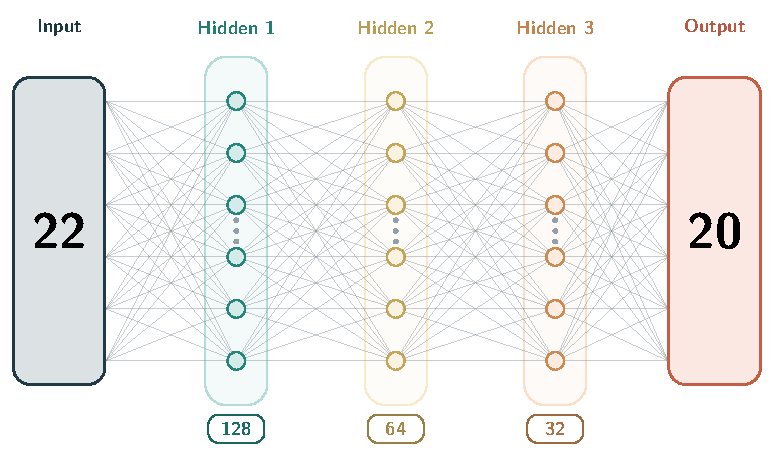
\includegraphics[width=\textwidth]{figure1_mlp_architecture.pdf}
\end{figrevr125}
\captionof{figure}{Architecture of the retained fully connected MLP baseline. The input and output stages are shown as labeled rectangular blocks to distinguish them from the hidden-layer neurons, which are shown as circular vertices. Representative vertices are displayed for the 22-input stage, the three hidden layers of widths 128, 64, and 32, and the 20-component effluent output stage, while the edge pattern indicates dense inter-layer connectivity between successive layers.}
\label{fig:mlp_architecture}
\end{center}
\end{revblockr125}

All retained models were assigned Optuna studies under a common tuning design (Akiba et al., 2019). Hyperparameter selection minimized validation mean squared error in the shared 20-component effluent prediction space using a seeded tree-structured Parzen estimator sampler (Bergstra et al., 2011), a no-pruning policy, and 100 trials per model. The authoritative 8,000-row training pool was first reduced to a 4,000-row tuning subset, corresponding to 50\% of the training pool, and that subset was then partitioned with a 20\% validation fraction, yielding 3,200 tuning-training rows and 800 tuning-validation rows. No wall-clock timeout was imposed. Once the Optuna studies were completed, the final selected hyperparameters were fixed and reused for the one-shot benchmark and the repeated dataset-size analysis.

\begin{table}[H]
\centering
\caption{Common Optuna design used for all retained models.}
\label{tab:optuna_design}
\scriptsize
\begin{tabular}{ll}
\hline
Setting & Value \\
\hline
Objective & Validation mean squared error \\
Optimization direction & Minimize \\
Sampler & Tree-structured Parzen estimator \\
Pruning policy & None \\
Study seed & 42 \\
Trials per model & 100 \\
Training-pool fraction for tuning & 0.50 \\
Validation fraction within tuning subset & 0.20 \\
Tuning-training rows & 3,200 \\
Tuning-validation rows & 800 \\
Timeout & None \\
\hline
\end{tabular}
\end{table}

\begin{table}[H]
\centering
\caption{Optuna-selected ICSOR hyperparameters.}
\label{tab:optuna_icsor}
\scriptsize
\begin{tabular}{ll}
\hline
Parameter & Selected value \\
\hline
include\_bias\_term & true \\
$\lambda_{inv}$ & $8.68 \times 10^{-3}$ \\
$\lambda_{sys}$ & $1.27 \times 10^{-3}$ \\
$\lambda_B$ & $6.09 \times 10^{-5}$ \\
$\lambda_{\Gamma}$ & $6.55 \times 10^{-4}$ \\
$\gamma_{abs}$ & 0.368 \\
max\_outer\_iterations & 60 \\
n\_restarts & 1 \\
objective\_regression\_window & 12 \\
objective\_regression\_slope\_tolerance & $2.85 \times 10^{-7}$ \\
\hline
\end{tabular}
\end{table}

\begin{table}[H]
\centering
\caption{Optuna-selected hyperparameters for the tree-based regressors.}
\label{tab:optuna_classical_a}
\scriptsize
\begin{tabular}{>{\raggedright\arraybackslash}p{2.1cm}>{\raggedright\arraybackslash}p{9.0cm}}
\hline
Model & Selected settings \\
\hline
XGBoost & $n_{estimators}=309$, learning\_rate$=0.125$, max\_depth$=3$, min\_child\_weight$=6.84$, subsample$=0.915$, colsample\_bytree$=0.828$, reg\_alpha$=1.18 \times 10^{-3}$, reg\_lambda$=0.382$ \\
LightGBM & $n_{estimators}=302$, learning\_rate$=0.0809$, num\_leaves$=16$, max\_depth$=8$, min\_child\_samples$=14$, subsample$=0.845$, colsample\_bytree$=0.869$, reg\_alpha$=3.17 \times 10^{-3}$, reg\_lambda$=3.36 \times 10^{-4}$ \\
CatBoost & iterations$=236$, learning\_rate$=0.172$, depth$=4$, l2\_leaf\_reg$=0.0266$, bagging\_temperature$=0.0277$, random\_strength$=0.0657$ \\
AdaBoost & $n_{estimators}=236$, learning\_rate$=0.999$, loss$=$square \\
Random Forest & $n_{estimators}=390$, max\_depth$=14$, min\_samples\_split$=3$, min\_samples\_leaf$=1$, max\_features$=0.500$, bootstrap$=$false \\
\hline
\end{tabular}
\end{table}

\begin{table}[H]
\centering
\caption{Optuna-selected hyperparameters for the kernel, instance-based, and linear regressors.}
\label{tab:optuna_classical_b}
\scriptsize
\begin{tabular}{>{\raggedright\arraybackslash}p{2.1cm}>{\raggedright\arraybackslash}p{9.0cm}}
\hline
Model & Selected settings \\
\hline
SVR & $C=0.118$, epsilon$=0.0458$, kernel$=$poly, gamma$=$scale, degree$=4$, tol$=8.96 \times 10^{-4}$, coef0$=0.889$ \\
$k$-NN & n\_neighbors$=15$, weights$=$distance, algorithm$=$kd\_tree, leaf\_size$=40$, $p=2$, metric$=$manhattan \\
PLS & n\_components$=6$, max\_iter$=887$, tol$=9.91 \times 10^{-5}$ \\
\hline
\end{tabular}
\end{table}

\begin{table}[H]
\centering
\caption{Optuna-selected hyperparameters for the retained fully connected ANN.}
\label{tab:optuna_mlp}
\scriptsize
\begin{tabular}{ll}
\hline
Parameter & Selected value \\
\hline
hidden\_layer\_sizes & (128, 64, 32) \\
activation & logistic \\
solver & adam \\
alpha & $6.33 \times 10^{-4}$ \\
batch\_size & 64 \\
learning\_rate\_init & $1.08 \times 10^{-3}$ \\
max\_iter & 500 \\
tol & $1.63 \times 10^{-5}$ \\
shuffle & false \\
early\_stopping & false \\
\hline
\end{tabular}
\end{table}
\end{revblockr24}

\begin{revblockr25}
\subsection{Evaluation Protocol}

A single row-wise 80--20 train-test split with random seed 42 was used for the one-shot benchmark, yielding 8,000 training rows and 2,000 test rows. The unconstrained regressors were standardized by z-score transformations fit on the training split only, separately for the 22-input feature matrix and the 20-output effluent-component matrix, to avoid preprocessing leakage from held-out data (Ba-Alawi et al., 2021; Pinheiro et al., 2025), and their predictions were inverse-transformed before external composite calculation and metric evaluation. ICSOR was kept in physical coordinates so that the invariant operator $A$, the coupled deployment rule, and the external reporting map $I_{comp}$ remained aligned with the formulation of Section~2. For all models, COD, TN, TP, and TSS were computed from the predicted component states through the same composition map, after which aggregate $R^2$, root mean squared error, mean absolute error, and mean absolute percentage error and per-target root mean squared error were reported over those four composites.

Only the final deployed component prediction of each model was used in the comparison. For ICSOR this is the constrained deployed component state, whereas for the classical regressors it is the direct unconstrained component prediction. Reported composite outputs were then obtained by applying the same external composition map to those final component states.

Sample-efficiency, computational scaling, and ranking stability were examined through a repeated dataset-size analysis based on repeated random train-test evaluations at each retained size. The 10,000-sample benchmark was subsampled without replacement at total sizes of 500, 1450, 2400, 3350, 4300, 5250, 6200, 7150, 8100, 9050, and 10,000 rows. At each retained total size, ten independent subsamples were drawn from the full benchmark using deterministic seeds derived from the base seed 42, and each subsample was split row-wise into an 80\% training partition and a 20\% held-out test partition using the same deterministic seed for that run. All ten retained models were trained and evaluated under the same size schedule, seed construction, and train-test fraction, so that observed performance differences at a given size reflect model structure rather than differences in protocol. This study contract yielded 110 train-test re-estimations per model across the full size sweep (11 retained sizes $\times$ 10 repeated runs per size). The Optuna-selected settings listed above were held fixed throughout this sweep so that the resulting learning curves isolated sample-size sensitivity and run-to-run variability rather than retuning noise. For every fit within this sweep, wall-clock training time was recorded, and computational scaling with dataset size was summarized from the distribution of training seconds across the ten repeated runs at each retained size. Predictive-performance ranking was based primarily on the mean held-out RMSE over the repeated runs, computed from the final reported composite outputs, and was supplemented by held-out MAE, MSE, MAPE, $R^2$, a normalized area-under-the-learning-curve summary, dense average rank across target-metric-size combinations, and the train-validation RMSE gap at the largest retained dataset size. Area-under-learning-curve summaries have prior use in the learning-curve and active-learning literature (Cawley, 2011; Guyon et al., 2011; Viering \& Loog, 2023). Here, a simple linear normalization over retained dataset size was used. Writing $\bar{M}_{i,m}(n)$ for the mean held-out metric of model $i$ at dataset size $n$ and metric $m$ over the repeated runs, the normalized area under the learning curve was computed by
\begin{equation}
\mathrm{nAUC}_{i,m} = \frac{1}{n_{\max} - n_{\min}} \int_{n_{\min}}^{n_{\max}} \bar{M}_{i,m}(n)\,dn,
\end{equation}
evaluated numerically by the trapezoidal rule over the sampled dataset sizes. For each metric $m$, target $k$, and size $n$, models were assigned a dense rank $r_{i,m,k}(n)$ from the mean held-out metric over repeated runs, with lower-is-better ordering for RMSE, MAE, MAPE, and MSE and higher-is-better ordering for $R^2$; this rank-based aggregation follows the same general benchmarking logic used for cross-dataset average-rank summaries in machine-learning evaluation (Dem\v{s}ar, 2006; Shevchenko et al., 2024), and the metric-specific average rank and overall average rank were then
\begin{equation}
\bar{r}_{i,m} = \frac{1}{KS} \sum_{k=1}^{K} \sum_{s=1}^{S} r_{i,m,k}(n_s),
\qquad
\bar{r}_{i} = \frac{1}{|\mathcal{M}|} \sum_{m \in \mathcal{M}} \bar{r}_{i,m},
\end{equation}
where $\mathcal{M} = \{\mathrm{RMSE},\mathrm{MAE},R^2,\mathrm{MAPE},\mathrm{MSE}\}$. At the largest retained dataset size $n_{\max}$, the train-validation RMSE gap was
\begin{equation}
\Delta_i^{\mathrm{RMSE}}(n_{\max}) = \overline{\mathrm{RMSE}}^{\mathrm{val}}_i(n_{\max}) - \overline{\mathrm{RMSE}}^{\mathrm{train}}_i(n_{\max}),
\end{equation}
so positive values indicate that the training partitions outperformed the held-out test partitions.

Physical-admissibility diagnostics were evaluated on the same final component-space predictions, because mass conservation and non-negativity are defined before external composition collapse. For a final component prediction $\tilde{c}$, mass-conservation violation was quantified by $v_{mc} = \|A(\tilde{c} - c_{in})\|_2$, and non-negativity violation was quantified by $v_{nn} = \|\min(\tilde{c}, 0)\|_1$, where the minimum is taken componentwise. A sample was counted as violating mass conservation or non-negativity when the corresponding quantity exceeded a numerical tolerance of $10^{-10}$. For each model, violation frequency was reported as the percentage of test samples that violated each condition.
\end{revblockr25}

\end{revblock}

\section{\rev{Results and Discussion}}
\begin{revblock}

\subsection{Overall Benchmark Performance on the Fixed Train-Test Split}

Table~\ref{tab:results_benchmark_sample} summarizes the fixed 80--20 benchmark after each model's predicted ASM component state has been collapsed through the same external composition map to COD, TN, TP, and TSS. Aggregate test RMSE is adopted as the primary ordering metric because it measures error in the same reported-composite space used throughout the comparison. On that criterion, the retained models separate into a leading group and a trailing group. The MLP attains the lowest aggregate RMSE (4.38), MAE (2.55), $R^2$ (0.9915), and MAPE (0.0123); LightGBM follows at RMSE 5.30; and SVR and ICSOR are closely spaced at 5.97 and 5.98, respectively.

\begin{table}[H]
\centering
\caption{Fixed-split 80--20 test performance of the retained model set in the reported-composite space. Metrics are computed after external composition collapse from the predicted ASM component states.}
\label{tab:results_benchmark_sample}
\scriptsize
\begin{tabular}{lcccc}
\hline
Model & RMSE & MAE & $R^2$ & MAPE \\
\hline
MLP & 4.38 & 2.55 & 0.9915 & 0.0123 \\
LightGBM & 5.30 & 3.21 & 0.9806 & 0.0203 \\
SVR & 5.97 & 3.49 & 0.9713 & 0.0244 \\
ICSOR & 5.98 & 3.70 & 0.9700 & 0.0256 \\
XGBoost & 6.10 & 3.79 & 0.9733 & 0.0243 \\
CatBoost & 6.45 & 4.07 & 0.9727 & 0.0250 \\
AdaBoost & 21.27 & 13.15 & 0.8643 & 0.0653 \\
$k$-NN & 23.61 & 13.87 & 0.8535 & 0.0557 \\
PLS & 28.24 & 17.05 & 0.7808 & 0.0681 \\
Random Forest & 29.00 & 16.93 & 0.7934 & 0.0632 \\
\hline
\end{tabular}
\end{table}

In terms of predictive accuracy on the fixed split, the MLP attains the lowest error among the retained baselines and LightGBM attains the lowest among the tree-based methods. ICSOR does not attain the lowest aggregate RMSE, but it remains within 0.68 of LightGBM and within 0.01 of SVR, while producing a lower aggregate RMSE than XGBoost and CatBoost. This placement is noteworthy because ICSOR operates under the physical constraints examined in Section~4.3, whereas the unconstrained baselines are not subject to conservation or non-negativity requirements during training or deployment.

Table~\ref{tab:results_target_sample} indicates that the aggregate ordering is driven primarily by COD, TN, and TSS. The MLP attains the lowest RMSE on all three of those composites, while LightGBM attains the lowest among the non-neural methods. On COD alone, ICSOR (RMSE 7.51) is within 0.06 of LightGBM and below XGBoost, CatBoost, SVR, and the remaining baselines. Its larger TN and TSS errors, however, prevent that COD performance from translating into a correspondingly favorable aggregate rank. TP contributes negligibly to model differentiation: every retained method falls within the narrow RMSE band 0.0811. The per-target decomposition therefore suggests that, once phosphorus prediction is effectively saturated, the observable model separation arises from carbon, nitrogen, and suspended-solids behavior.

\begin{table}[htbp]
\centering
\caption{Per-target fixed-split test RMSE for the retained models in the reported-composite space.}
\label{tab:results_target_sample}
\scriptsize
\begin{tabular}{lcccc}
\hline
Model & COD & TN & TP & TSS \\
\hline
MLP & 6.80 & 1.53 & 0.0811 & 6.06 \\
LightGBM & 7.45 & 2.73 & 0.0811 & 6.93 \\
SVR & 8.47 & 3.45 & 0.0811 & 7.25 \\
ICSOR & 7.51 & 3.53 & 0.0811 & 8.49 \\
XGBoost & 8.61 & 3.20 & 0.0811 & 8.03 \\
CatBoost & 8.80 & 3.13 & 0.0811 & 8.34 \\
AdaBoost & 38.44 & 5.40 & 0.0811 & 18.11 \\
$k$-NN & 38.53 & 4.18 & 0.0811 & 27.48 \\
PLS & 42.31 & 5.07 & 0.0811 & 36.20 \\
Random Forest & 45.28 & 3.91 & 0.0811 & 35.32 \\
\hline
\end{tabular}
\end{table}

Because the leading fixed-split models remain closely spaced on aggregate RMSE, a single train-test partition does not suffice to characterize sample efficiency or ranking stability. The repeated dataset-size study described below provides a broader basis for distinguishing models whose performance on one split may not generalize from those that remain competitive as the amount of training data varies.

\begin{revblockr25}
\subsection{Sample Efficiency, Ranking Stability, and Generalization}

Figure~\ref{fig:results_learning_curve_sample} shows a pattern that the fixed split alone does not capture: at the smallest retained dataset size of 500 rows, ICSOR attains the lowest mean held-out RMSE (10.79) among the retained models, followed by XGBoost (11.26) and LightGBM (11.45), while the MLP ranks fifth (13.26). As dataset size increases, however, the ordering shifts. By the full 10,000-row dataset size, the MLP attains the lowest RMSE (4.62), followed by LightGBM (5.27), SVR (5.84), and ICSOR (5.94). This crossover is consistent with broader learning-curve and hybrid-modeling literature, in which models with stronger structural priors can be more sample-efficient at small $N$, whereas more flexible unconstrained models may overtake them once sufficient data are available (Viering \& Loog, 2023; Shen et al., 2023).

\begin{figure}
\centering
\begin{figrevr25}
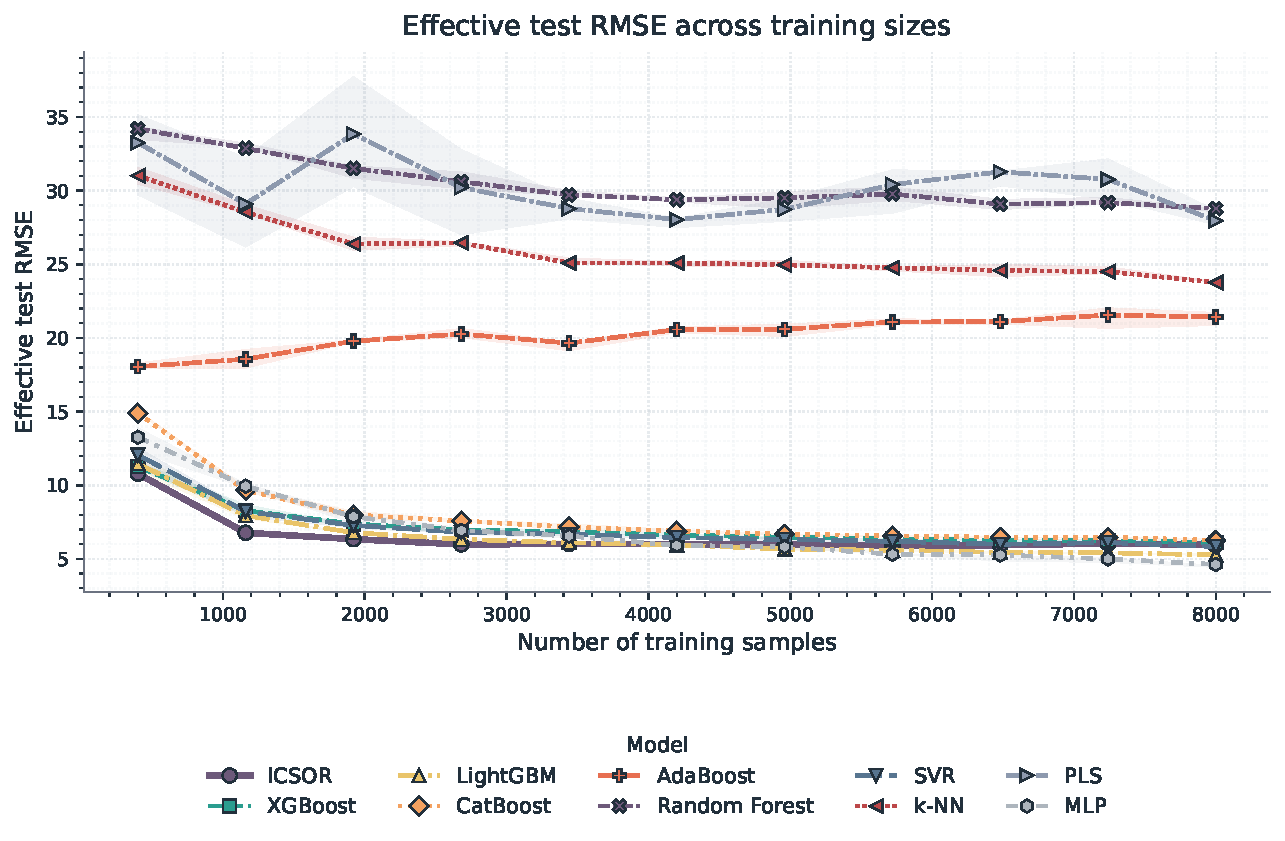
\includegraphics[width=0.92\textwidth]{figure2_rmse_learning_curve.pdf}
\end{figrevr25}
\caption{Repeated dataset-size learning curves from the repeated random train-test evaluations at each retained size. Lines show the mean held-out RMSE across the retained dataset-size sweep, and shaded bands show the interquartile range across the ten repeated runs at each size.}
\label{fig:results_learning_curve_sample}
\end{figure}

Table~\ref{tab:results_scaling_sample} condenses the repeated-size sweep into four summary statistics. ICSOR attains the lowest RMSE nAUC (6.33), indicating that its average RMSE profile across the full range of retained dataset sizes is favorable even though it does not attain the lowest final-size RMSE. LightGBM attains the lowest sample-average rank (2.2) and the MLP is second (2.5), indicating that when the evaluation is broadened across all reported metrics, targets, and retained dataset sizes, the unconstrained baselines with the lowest pointwise errors also tend to rank well on a broader set of criteria. ICSOR's sample-average rank of 4.3 is comparable to that of XGBoost (4.3), suggesting that its low-data advantage, while observable, does not translate into a dominant rank across the full evaluation grid.

\begin{table}[htbp]
\centering
\caption{Summary of the repeated dataset-size benchmark. Final RMSE and $\Delta$RMSE are evaluated at the largest retained dataset size, and lower values are better for all columns except that a smaller $\Delta$RMSE indicates less train-validation separation.}
\label{tab:results_scaling_sample}
\scriptsize
\begin{tabular}{lcccc}
\hline
Model & Final RMSE & RMSE nAUC & Sample Avg. Rank & $\Delta$RMSE \\
\hline
MLP & 4.62 & 6.75 & 2.5 & 0.65 \\
LightGBM & 5.27 & 6.35 & 2.2 & 1.99 \\
SVR & 5.84 & 6.90 & 4.0 & 1.19 \\
ICSOR & 5.94 & 6.33 & 4.3 & 0.22 \\
XGBoost & 6.10 & 7.01 & 4.3 & 1.44 \\
CatBoost & 6.26 & 7.60 & 5.0 & 0.69 \\
AdaBoost & 21.42 & 20.29 & 8.2 & 0.23 \\
$k$-NN & 23.76 & 25.77 & 7.0 & 23.66 \\
PLS & 27.96 & 30.17 & 9.4 & 0.38 \\
Random Forest & 28.78 & 30.31 & 8.2 & 18.71 \\
\hline
\end{tabular}
\end{table}

The generalization behavior observed in Table~\ref{tab:results_scaling_sample} warrants separate attention. The train-validation RMSE gap of ICSOR at the largest retained dataset size is 0.22, which is the smallest among the competitively accurate models and considerably lower than those of LightGBM (1.99), XGBoost (1.44), SVR (1.19), and the MLP (0.65). PLS also exhibits a small gap (0.38), but its training and held-out errors are both large, consistent with the high-bias, low-variance pattern classically associated with underfitting and with prior evidence that linear PLS can mis-specify strongly nonlinear wastewater behavior (Geman et al., 1992; Woo et al., 2009). This pattern is consistent with broader physics-informed and constrained-learning evidence that structural restrictions can improve generalization and data efficiency by restricting the admissible solution space (Hansen et al., 2024; Kashinath et al., 2021). In the present benchmark, the repeated-size analysis therefore suggests that the structural restrictions imposed by ICSOR tend to reduce overfitting relative to the unconstrained baselines without a proportionate loss in predictive accuracy; at the full 10,000-row dataset scale the model remains within the range of SVR and XGBoost while exhibiting a smaller train-validation separation.

Figure~\ref{fig:results_runtime_sample} shows that this favorable generalization comes at a cost in training time. At the smallest retained dataset size of 500 rows, ICSOR requires a mean of 21.5~s, compared with 4.72~s for LightGBM, 3.16~s for XGBoost, and 4.99~s for the MLP. At the full 10,000-row dataset size, ICSOR rises to 94.4~s, which is slower than the tree-based models (4.13--8.13~s), PLS (0.228~s), and $k$-NN (2.70~s), but remains below AdaBoost (117.7~s), SVR (136.8~s), and the MLP (161.6~s). The recursive coupled-QP route is therefore more expensive than the fastest retained methods at every retained size, but it does not become the costliest option at the larger dataset scales and remains practical for offline surrogate fitting.

\begin{figure}
\centering
\begin{figrevr25}
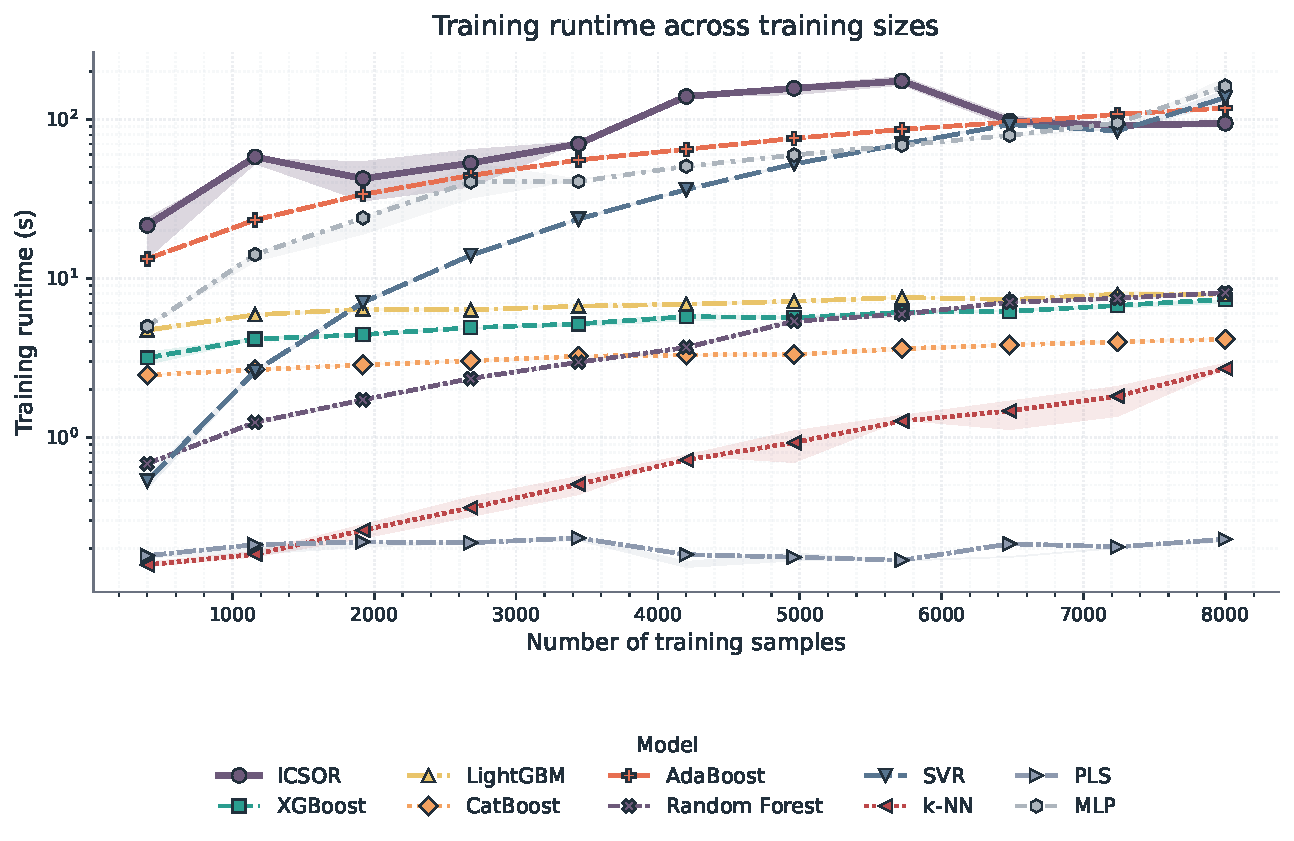
\includegraphics[width=0.92\textwidth]{figure3_runtime_learning_curve.pdf}
\end{figrevr25}
\caption{Repeated dataset-size runtime curves for the retained models. Lines show the mean training time across repeated runs and shaded bands show the interquartile range across the ten repeated runs at each size; the y-axis is logarithmic to keep the full cost spread readable.}
\label{fig:results_runtime_sample}
\end{figure}
\end{revblockr25}

\begin{revblockr22}
\subsection{Physical Admissibility and Deployment Behavior}

Table~\ref{tab:results_physical_sample} reports the physical-admissibility outcome. ICSOR is the only retained model that produces 0.0\% mass-conservation violations and 0.0\% non-negativity violations on the final component-space test predictions. Every unconstrained baseline violates conservation on 100\% of the test samples. Non-negativity violation frequencies vary across models, ranging from 0.0\% for AdaBoost, Random Forest, and $k$-NN to 70.1\% for CatBoost, 68.65\% for SVR, 64.05\% for XGBoost, 58.2\% for the MLP, 48.7\% for PLS, and 46.0\% for LightGBM.

The zero non-negativity frequency for AdaBoost, Random Forest, and $k$-NN should not be interpreted as full physical admissibility. These regressors still violate the invariant conservation relations on every test sample, but their componentwise predictions are formed through aggregation rules that can preserve non-negativity when trained on nonnegative concentration targets: Random Forest averages nonnegative leaf responses, $k$-NN averages nonnegative neighbor responses, and AdaBoost combines nonnegative tree responses through a weighted-median ensemble rule. Their reported 0.0\% non-negativity rate therefore reflects the geometry of these unconstrained predictors in the positive orthant, not enforcement of stoichiometric feasibility.

\begin{table}[htbp]
\centering
\caption{Physical-admissibility violation frequencies evaluated on the final component-space test predictions. Mass conservation and non-negativity are assessed before external composition collapse.}
\label{tab:results_physical_sample}
\scriptsize
\begin{tabular}{lcc}
\hline
Model & Mass-Conservation Violations (\%) & Non-Negativity Violations (\%) \\
\hline
MLP & 100.0 & 58.20 \\
LightGBM & 100.0 & 46.00 \\
SVR & 100.0 & 68.65 \\
ICSOR & 0.0 & 0.0 \\
XGBoost & 100.0 & 64.05 \\
CatBoost & 100.0 & 70.10 \\
AdaBoost & 100.0 & 0.0 \\
$k$-NN & 100.0 & 0.0 \\
PLS & 100.0 & 48.70 \\
Random Forest & 100.0 & 0.0 \\
\hline
\end{tabular}
\end{table}

These diagnostics illustrate why predictive accuracy in the reported composite space does not by itself ensure physically interpretable component-level predictions. AdaBoost, Random Forest, and $k$-NN remain nonnegative on the test set, yet all three still violate the stoichiometric invariants on every sample; positivity alone therefore does not recover consistent material bookkeeping. Conversely, several of the models with the lowest aggregate RMSE, including the MLP and LightGBM, violate the conserved material inventories on every test sample and produce negative component concentrations on a substantial fraction of the test set. A surrogate may thus appear accurate in the reported composite space while producing component-level states that are not physically admissible, a mismatch that has also been documented in atmospheric-composition and reaction-kinetics surrogates when favorable aggregate error metrics obscure physically unacceptable species- or component-level behavior (Kircher \& Votsmeier, 2025; Sturm \& Silva, 2025).

The staged deployment logic of ICSOR can also be examined at the level of individual correction stages. None of the raw coupled test predictions were simultaneously invariant-consistent and nonnegative: raw feasibility was 0.0\%, raw conservation compliance was 0.0\%, and 21.7\% of raw states were nonnegative. The closed-form affine projection restored invariants for all samples and was itself sufficient for 21.8\% of the test set (436 of 2000 samples), resolving those cases without invoking any numerical optimizer. The remaining 78.2\% (1564 samples) required the final LP correction, which converged in a mean of 23.5 HiGHS iterations with a maximum of 40. The final projected prediction was feasible for 100\% of the test cases, confirming that the deployment pipeline maintained the physical guarantees without requiring a computationally expensive solve on every sample.

Taken together, these results suggest a moderate accuracy-feasibility tradeoff within the present benchmark, consistent with prior physics-informed ML studies showing that exact conservation enforcement or hard corrective constraints can improve physical admissibility while sometimes sacrificing pointwise predictive accuracy (Hansen et al., 2024; Sturm \& Silva, 2025). When the objective is minimizing pointwise error in the reported composite space, the MLP and LightGBM remain the preferable options. When the objective includes deployed predictions that satisfy both invariant conservation and component non-negativity, ICSOR is the only model in the retained set that provides those guarantees, and it does so while remaining within the upper portion of the competitive accuracy range on aggregate RMSE.
\end{revblockr22}

\begin{revblockr21}
\subsection{Interpretable Structure of the Learned ICSOR Model}

Figure~\ref{fig:results_interpretability_sample} presents the COD-specific $\Theta_{cc}$ block extracted from the fitted ICSOR driver. The full COD, TN, TP, and TSS atlases are provided as Supplementary Figures S1--S4. The main manuscript presents this COD panel because it provides a direct view of how influent-influent curvature is allocated once the operational main effects, influent main effects, and coupling matrix have absorbed the lower-order structure.

\begin{figure}
\centering
\begin{figrevr21}
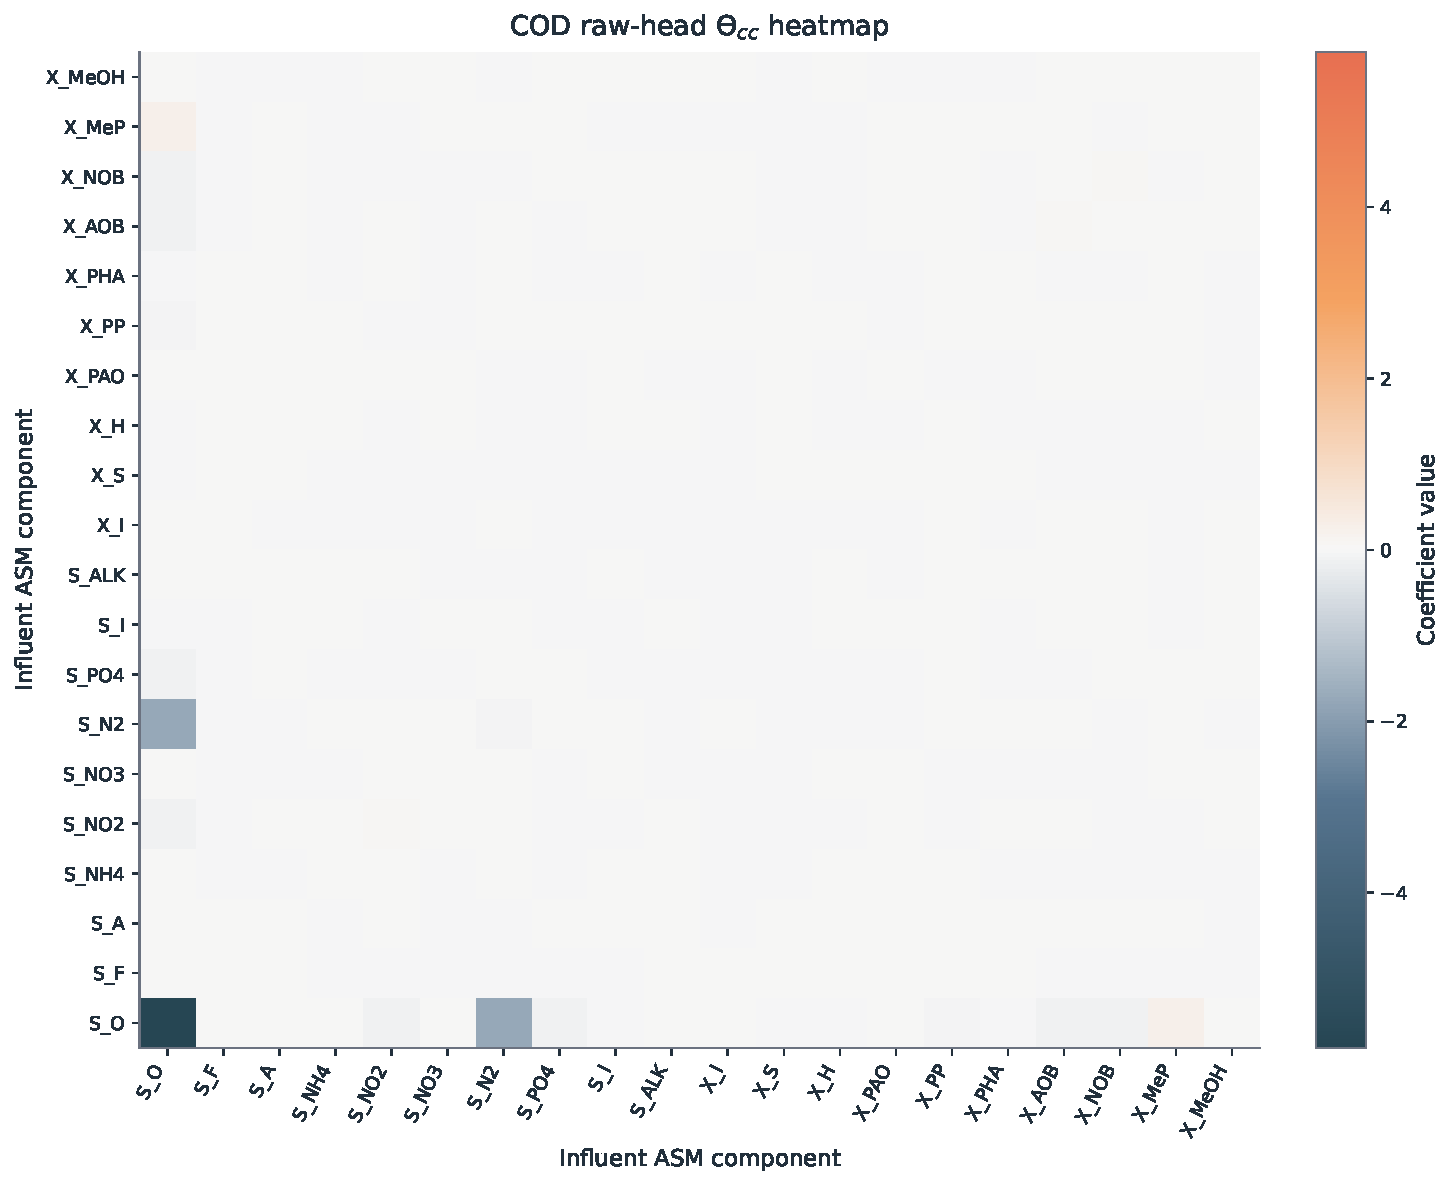
\includegraphics[width=0.94\textwidth]{figure4_icsor_structure.pdf}
\end{figrevr21}
\caption{COD-specific $\Theta_{cc}$ heatmap from the fitted ICSOR driver. Rows and columns enumerate the influent ASM components, and color encodes the sign and magnitude of the second-order COD curvature. The full COD, TN, TP, and TSS target atlases are reported in Supplementary Figures S1--S4.}
\label{fig:results_interpretability_sample}
\end{figure}

The retained COD interactions are concentrated around dissolved oxygen and nitrogen-linked states rather than spread uniformly across all 400 possible influent-pair entries. The largest-magnitude coefficient is the negative $S_O$--$S_O$ self-curvature term ($-2.3899 \times 10^{-2}$), followed by the symmetric negative cross-interactions $S_O$--$S_{N2}$ and $S_O$--$S_{NO2}$ ($-2.1845 \times 10^{-2}$ and $-1.4691 \times 10^{-2}$, respectively). Smaller terms link $S_O$ to $X_{NOB}$, $X_{AOB}$, $X_{MeOH}$, and $X_{PP}$, while positive diagonal curvature appears for $S_{N2}$, $X_{AOB}$, and $X_{NOB}$. In engineering terms, the fitted COD driver indicates that second-order COD behavior in this reactor is associated primarily with the redox environment and nitrifier-linked loading interactions rather than with a broad field of carbon-only cross terms, consistent with established activated-sludge evidence that dissolved oxygen enters ASM kinetics through nonlinear switching functions, mediates carbon-oxidation and nitrification tradeoffs, and remains a primary operational variable linking aeration demand to nitrogen-conversion behavior (Henze et al., 2006; Stenstrom \& Song, 1991; de Araujo et al., 2013; Wentzel et al., 1992).

\begin{table}[htbp]
\centering
\caption{COD blockwise retained-coefficient counts using the export threshold ($10^{-4}$ of the maximum absolute coefficient magnitude) applied in the comparison notebook. The table summarizes which fitted coefficients remain materially active in the reported COD structure.}
\label{tab:results_icsor_regularization_sample}
\scriptsize
\setlength{\tabcolsep}{4pt}
\begin{tabular}{p{3.0cm}p{2.1cm}p{2.4cm}p{2.0cm}}
\hline
Coefficient block & Total coeffs. & Retained coeffs. & \% Retained \\
\hline
$b$ & 1 & 1 & 100.0 \\
$W_u$ & 2 & 2 & 100.0 \\
$W_{in}$ & 20 & 20 & 100.0 \\
$\Theta_{uu}$ & 4 & 4 & 100.0 \\
$\Theta_{uc}$ & 40 & 18 & 45.0 \\
$\Theta_{cc}$ & 400 & 59 & 14.8 \\
$\Gamma$ & 380 & 356 & 93.7 \\
Overall summary & 847 & 460 & 54.3 \\
\hline
\end{tabular}
\end{table}

Table~\ref{tab:results_icsor_regularization_sample} shows that this interpretability does not arise from a uniformly sparse model, but from a structured separation between sparse high-order driver terms and a comparatively dense cross-component coupling layer. \revitem{revRtwoOne}{The export threshold used to classify a fitted coefficient as retained is $10^{-4}$ of the maximum absolute coefficient magnitude within each target; coefficients below this threshold are treated as numerically negligible for reporting purposes. This threshold is a post-training reporting rule only: it does not affect model selection, training, or deployment, and serves solely to distinguish materially active coefficients from those whose magnitude is too small to warrant physical interpretation.} Under the COD export threshold, every low-dimensional block is retained in full ($b$, $W_u$, $W_{in}$, and $\Theta_{uu}$), whereas only 18 of 40 $\Theta_{uc}$ terms and 59 of 400 $\Theta_{cc}$ terms remain above the reporting threshold. By contrast, 356 of 380 $\Gamma$ entries are retained. The model therefore compresses nonlinear influent curvature while preserving a broad redistribution layer across ASM components. Overall, 54.3\% of the candidate coefficients remain above the reporting threshold, and most of that retained fraction resides in the coupling matrix rather than in the highest-order quadratic block. This retention pattern is consistent with structured-sparsity formulations that suppress higher-order terms while preserving coupling across meaningful variable groups (Yuan \& Lin, 2006; Bach et al., 2012).

This separation between a sparse quadratic driver and a comparatively dense coupling matrix is why Figure~\ref{fig:results_interpretability_sample} can present a compact curvature surface without omitting important model structure. The COD $\Theta_{cc}$ panel serves as the representative interpretability surface, while Supplementary Figures S1--S4 preserve the full target-by-target atlases for completeness. Presenting the main discussion at the COD-block level therefore highlights the curvature structure that is most relevant to process interpretation while acknowledging that the complete ICSOR coefficient structure is distributed across $B$ and $\Gamma$ together; in this setting, inspection of coefficient signs, magnitudes, and block patterns is part of the scientific interpretation rather than a separate explanatory layer (Brunton et al., 2016; Shen et al., 2023).

\revitem{revRtwoOne}{This coefficient-level interpretation differs qualitatively from what PLS or ANN sensitivity analysis provides. PLS loading weights identify linear latent directions that maximize covariance between inputs and outputs, but they are fitted without any physical-admissibility requirement and cannot separate operating effects, loading effects, within-subspace curvature, and cross-component coupling into distinct named blocks. ANN sensitivity analyses are local, post hoc response diagnostics that describe how a trained prediction changes with a small input perturbation; they do not expose the global model structure and are derived from parameters fitted without conservation or positivity enforcement. By contrast, the ICSOR coefficient blocks are explicit global model parameters whose values are shaped by the requirement that the resulting predictions must satisfy stoichiometric mass conservation and componentwise non-negativity. Because none of the benchmark models impose such constraints during training, the learned ICSOR coefficients are structurally constrained to produce only physically admissible redistributions, which gives the resulting interaction signs and magnitudes a more physically grounded basis for process interpretation.}

\revitem{revRtwoFour}{The coefficients presented in Figure~\ref{fig:results_interpretability_sample} and Table~\ref{tab:results_icsor_regularization_sample} correspond to a single ICSOR fit on the full training partition, not to an aggregate across multiple fits. Because ICSOR is a data-driven statistical model, its fitted coefficients are expected to vary across different training samples. The recursive coupled-QP estimator described in Section~2.6 minimizes a non-convex joint objective over $(B, \Gamma, \widehat{C})$ through block-coordinate sweeps with restarts, and the non-convexity of that joint problem means that the estimator does not guarantee a unique global minimum: different initializations, restart outcomes, and training partitions can lead to distinct stationary points with comparable objective values. Furthermore, the coupling matrix $\Gamma$ and the driver matrix $B$ can trade off against each other in the coupled relation $Rc = B\phi$, so different $(B, \Gamma)$ pairs may produce similar fitted component states and predictive accuracy while differing in their individual coefficient values. This identifiability limitation is a property of the model class rather than a defect of the estimation procedure, and it is shared by many transparent model families including linear regression on collinear features, sparse polynomial models, and structured equation-learning approaches (Brunton et al., 2016). Physical interpretation should therefore focus on persistent structural patterns---such as which blocks are sparse, which interaction signs are stable, and which coupling pathways recur---rather than on the precise numerical value of any single coefficient. Quantifying coefficient-level stability across repeated resamples remains an open diagnostic that future work should address.}
\end{revblockr21}

\end{revblock}

\section{\rev{Conclusion}}

\begin{revblock}

This study developed Invariant-Constrained Second-Order Regression (ICSOR), an interpretable surrogate framework for steady-state activated sludge systems that enforces exact stoichiometric mass conservation and componentwise non-negativity within a single formulation. The framework combines a partitioned second-order feature map, a learned cross-component coupling matrix, deterministic recursive coupled-QP estimation, and a hierarchical deployment correction consisting of a raw feasibility check, a closed-form affine invariant projection, and a final linear program. In the ASM2d-TSN continuous stirred tank reactor benchmark examined here, ICSOR was the only retained model that produced no mass-conservation violations and no non-negativity violations on the final component-space test predictions, whereas every unconstrained baseline violated conservation on all test samples and several exhibited negative component concentrations on a substantial fraction of the test set.

These physical guarantees were obtained with a moderate predictive tradeoff. On the fixed 80--20 split, ICSOR attained an aggregate test RMSE of 5.98 in the reported composite space, which remained within the range of SVR and XGBoost but did not match the lower errors achieved by the MLP (4.38) and LightGBM (5.30) when unconstrained accuracy alone was the criterion. In the repeated dataset-size study, ICSOR attained the lowest mean held-out RMSE at the smallest retained dataset size and the lowest RMSE normalized area under the learning curve across the full size sweep, while exhibiting the smallest train-validation RMSE gap (0.22) among the competitively accurate models. Training cost was higher than that of the fastest tree-based methods at every retained size, though it remained below that of SVR and the MLP at the largest dataset scale.

The conclusions drawn here are bounded by the scope of the present study. The framework was validated only on steady-state predictions from a standalone CSTR operating within the sampled influent and operating-condition ranges, and it does not claim to enforce full kinetic or thermodynamic feasibility. The invariant matrix used for conservation enforcement depends on the adopted stoichiometric model and system boundary, so any external source or sink not represented in that model lies outside the present conservation claim. Within these boundaries, the results suggest that physically admissible surrogate predictions can be maintained without forgoing interpretability or incurring a disproportionate loss in predictive accuracy. Whether this tradeoff remains favorable for more complex reactor configurations, broader operating envelopes, or integration into surrogate-assisted optimization and control workflows, where surrogate-based prediction has already shown promise for wastewater optimization and control, remains to be investigated for invariant-constrained surrogates in future work (Sadeghassadi et al., 2018; Wang et al., 2025).
\end{revblock}

\section*{CRediT authorship contribution statement}

The sole author, Egberto F. Selerio Jr., contributed to conceptualization, methodology, software, validation, formal analysis, investigation, resources, data curation, writing---original draft, writing---review \& editing, visualization, supervision, project administration, and funding acquisition.

\section*{Acknowledgments \& disclosure of funding}

This work is funded by the Department of Science and Technology of the Philippines through the Engineering Research and Development for Technology scholarship awarded to Egberto F. Selerio Jr. at the University of San Carlos.

\section*{Data availability}

The complete codebase that reproduces the results presented in this study is available in the GitHub repository \texttt{https://github.com/egbertoselerio1997/icsor.git}. The repository may be cloned using the command \texttt{git clone https://github.com/egbertoselerio1997/icsor.git}.

\section*{References}

\noindent Aboagye, E. A., Burnham, S. M., Dailey, J., Zia, R., Tran, C., Desai, M., \& Yenkie, K. M. (2021). Systematic design, optimization, and sustainability assessment for generation of efficient wastewater treatment networks. \textit{Water, 13}(9), 1326.

\noindent de Araujo, A. C. B., Gallani, S., Mulas, M., \& Skogestad, S. (2013). Sensitivity analysis of optimal operation of an activated sludge process model for economic controlled variable selection. \textit{Industrial \& Engineering Chemistry Research, 52}(29), 9908--9921.

\noindent Ahn, J. Y., Chu, K. H., Yoo, S. S., Mang, J. S., Sung, B. W., \& Ko, K. B. (2014). Determination of optimal operating factors via modeling for livestock wastewater treatment: Comparison of simulated and experimental data. \textit{International Biodeterioration \& Biodegradation, 95}, 46--54.

\noindent Akiba, T., Sano, S., Yanase, T., Ohta, T., \& Koyama, M. (2019). Optuna: A next-generation hyperparameter optimization framework. In \textit{Proceedings of the 25th ACM SIGKDD International Conference on Knowledge Discovery \& Data Mining} (pp. 2623--2631).

\noindent Asadi, A., Verma, A., Yang, K., \& Mejabi, B. (2017). Wastewater treatment aeration process optimization: A data mining approach. \textit{Journal of Environmental Management, 203}, 630--639.

\noindent Bach, F., Jenatton, R., Mairal, J., \& Obozinski, G. (2012). Optimization with sparsity-inducing penalties. \textit{Foundations and Trends in Machine Learning, 4}(1), 1--106.

\noindent Bagherzadeh, F., Mehrani, M. J., Basirifard, M., \& Roostaei, J. (2021). Comparative study on total nitrogen prediction in wastewater treatment plant and effect of various feature selection methods on machine learning algorithms performance. \textit{Journal of Water Process Engineering, 41}, 102033.

\noindent Ba-Alawi, A. H., Vilela, P., Loy-Benitez, J., Heo, S., \& Yoo, C. (2021). Intelligent sensor validation for sustainable influent quality monitoring in wastewater treatment plants using stacked denoising autoencoders. \textit{Journal of Water Process Engineering, 43}, 102206.

\noindent Bergstra, J., Bardenet, R., Bengio, Y., \& K\'egl, B. (2011). Algorithms for hyper-parameter optimization. In \textit{Advances in Neural Information Processing Systems} (Vol. 24).

\noindent Beucler, T., Pritchard, M., Rasp, S., Ott, J., Baldi, P., \& Gentine, P. (2021). Enforcing analytic constraints in neural networks emulating physical systems. \textit{Physical Review Letters, 126}(9), 098302.

\noindent Brunton, S. L., Proctor, J. L., \& Kutz, J. N. (2016). Discovering governing equations from data by sparse identification of nonlinear dynamical systems. \textit{Proceedings of the National Academy of Sciences, 113}(15), 3932--3937.

\noindent Bhosekar, A., \& Ierapetritou, M. (2018). Advances in surrogate based modeling, feasibility analysis, and optimization: A review. \textit{Computers \& Chemical Engineering, 108}, 250--267.

\noindent Croll, H. C., Ikuma, K., Ong, S. K., \& Sarkar, S. (2023). Reinforcement learning applied to wastewater treatment process control optimization: Approaches, challenges, and path forward. \textit{Critical Reviews in Environmental Science and Technology, 53}(20), 1775--1794.

\noindent Curtiss, C. F., \& Hirschfelder, J. O. (1952). Integration of stiff equations. \textit{Proceedings of the National Academy of Sciences, 38}(3), 235--243.

\noindent Cawley, G. C. (2011). Baseline methods for active learning. \textit{JMLR Workshop and Conference Proceedings, 16}, 47--57.

\noindent Dem\v{s}ar, J. (2006). Statistical comparisons of classifiers over multiple data sets. \textit{Journal of Machine Learning Research, 7}, 1--30.

\noindent Duan, S., Zhang, Y., \& Zheng, S. (2022). Heterotrophic nitrifying bacteria in wastewater biological nitrogen removal systems: A review. \textit{Critical Reviews in Environmental Science and Technology, 52}(13), 2302--2338.

\noindent Durkin, A., Otte, L., \& Guo, M. (2024). Surrogate-based optimisation of process systems to recover resources from wastewater. \textit{Computers \& Chemical Engineering, 182}, 108584.

\noindent Fang, F., Ni, B., Li, W., Sheng, G., \& Yu, H. (2011). A simulation-based integrated approach to optimize the biological nutrient removal process in a full-scale wastewater treatment plant. \textit{Chemical Engineering Journal, 174}(2--3), 635--643.

\noindent Geiss, A., Silva, S. J., \& Hardin, J. C. (2022). Downscaling atmospheric chemistry simulations with physically consistent deep learning. \textit{Geoscientific Model Development, 15}(17), 6677--6694.

\noindent Geman, S., Bienenstock, E., \& Doursat, R. (1992). Neural networks and the bias\/variance dilemma. \textit{Neural Computation, 4}(1), 1--58.

\noindent Guyon, I., Cawley, G., Dror, G., \& Lemaire, V. (2011). Results of the active learning challenge. \textit{JMLR Workshop and Conference Proceedings, 16}, 19--45.

\noindent Guerrero, J., Guisasola, A., \& Baeza, J. A. (2011). The nature of the carbon source rules the competition between PAO and denitrifiers in systems for simultaneous biological nitrogen and phosphorus removal. \textit{Water Research, 45}(16), 4793--4802.

\noindent Harder, P., Watson-Parris, D., Stier, P., Strassel, D., Gauger, N. R., \& Keuper, J. (2022). Physics-informed learning of aerosol microphysics. \textit{Environmental Data Science, 1}, e20.

\noindent Hansen, D., Maddix, D. C., Alizadeh, S., Gupta, G., \& Mahoney, M. W. (2024). Learning physical models that can respect conservation laws. \textit{Physica D: Nonlinear Phenomena, 457}, 133952.

\noindent Huangfu, Q., \& Hall, J. A. J. (2018). Parallelizing the dual revised simplex method. \textit{Mathematical Programming Computation, 10}(1), 119--142.

\noindent Henze, M., Gujer, W., Mino, T., \& van Loosedrecht, M. (2006). Activated Sludge Models ASM1, ASM2, ASM2d and ASM3. \textit{Water Intelligence Online, 5}(0).

\noindent Henze, M., Gujer, W., Mino, T., Matsuo, T., Wentzel, M. C., Marais, G. v. R., \& van Loosdrecht, M. C. M. (1999). Activated Sludge Model No. 2d, ASM2D. \textit{Water Science and Technology, 39}(1), 165--182.

\noindent Khatri, P., Gupta, K. K., \& Gupta, R. K. (2020). A review of partial least squares modeling (PLSM) for water quality analysis. \textit{Modeling Earth Systems and Environment, 6}, 1419--1426.

\noindent Kim, M., Rao, A. S., \& Yoo, C. (2009). Dual Optimization Strategy for N and P Removal in a Biological Wastewater Treatment Plant. \textit{Industrial and Engineering Chemistry Research, 48}(13), 6363--6371.

\noindent Kircher, T., \& Votsmeier, M. (2025). Machine learning surrogate models for mechanistic kinetics: Embedding atom balance and positivity. \textit{The Journal of Physical Chemistry Letters, 16}(19), 4715--4723.

\noindent Kashinath, K., Mustafa, M., Albert, A., Wu, J.-L., Jiang, C., Esmaeilzadeh, S., Azizzadenesheli, K., Wang, R., Chattopadhyay, A., Singh, A., Manepalli, A., Chirila, D., Yu, R., Walters, R., White, B., Xiao, H., Tchelepi, H. A., Marcus, P., Anandkumar, A., Hassanzadeh, P., \& Prabhat. (2021). Physics-informed machine learning: Case studies for weather and climate modelling. \textit{Philosophical Transactions of the Royal Society A: Mathematical, Physical and Engineering Sciences, 379}(2194), 20200093.

\noindent Li, M., Hu, S., Xia, J., Wang, J., Song, X., \& Shen, H. (2020). Dissolved Oxygen Model Predictive Control for Activated Sludge Process Model Based on the Fuzzy C-means Cluster Algorithm. \textit{International Journal of Control, Automation and Systems, 18}(9), 2435--2444.

\noindent Lim, J., Lee, Y., Ataei, A., \& Yoo, C. (2011). Exploration of dual optimal conditions for COD and nitrogen removal in an MBR. \textit{Asia-Pacific Journal of Chemical Engineering, 6}(3), 433--440.

\noindent Lin, L., Yang, H., \& Xu, X. (2022). Effects of Water Pollution on Human Health and Disease Heterogeneity: A Review. \textit{Frontiers in Environmental Science, 10}, 880246.

\noindent Liu, H., Yang, J., Zhang, Y., \& Yang, C. (2021). Monitoring of wastewater treatment processes using dynamic concurrent kernel partial least squares. \textit{Process Safety and Environmental Protection, 147}, 274--282.

\noindent Madhav, S., Ahamad, A., Singh, A. K., Kushawaha, J., Chauhan, J. S., Sharma, S., \& Singh, P. (2020). \textit{Water pollutants: sources and impact on the environment and human health}. In \textit{Sensors in Water Pollutants Monitoring: Role of Material}, 43--62.

\noindent Machado, V. C., Lafuente, J., \& Baeza, J. A. (2014). Activated sludge model 2d calibration with full-scale WWTP data: comparing model parameter identifiability with influent and operational uncertainty. \textit{Bioprocess and Biosystems Engineering, 37}(7), 1271--1287.

\noindent McKay, M. D., Beckman, R. J., \& Conover, W. J. (1979). Comparison of three methods for selecting values of input variables in the analysis of output from a computer code. \textit{Technometrics, 21}(2), 239--245.

\noindent Mao, Z., Li, X., Zhang, X., Li, D., Lu, J., Li, J., \& Zheng, F. (2024). Optimization of effluent quality and energy consumption of aeration process in wastewater treatment plants using artificial intelligence. \textit{Journal of Water Process Engineering, 63}, 105384.

\noindent Min, Y., Sonar, A., \& Azizan, N. (2024). Hard-constrained neural networks with universal approximation guarantees. \textit{arXiv preprint arXiv:2410.10807}.

\noindent Nazlabadi, E., Niaragh, E. K., \& Moghaddam, M. R. A. (2021). A systematic and critical review of two decades' application of response surface methodology in biological wastewater treatment processes. \textit{Desalination and Water Treatment, 228}, 92--120.

\noindent Newhart, K. B., Holloway, R. W., Hering, A. S., \& Cath, T. Y. (2019). Data-driven performance analyses of wastewater treatment plants: A review. \textit{Water Research, 157}, 498--513.

\noindent Padron-Paez, J. I., Almaraz, S. D. L., \& Rom\'an-Mart\'inez, A. (2020). Sustainable wastewater treatment plants design through multiobjective optimization. \textit{Computers \& Chemical Engineering, 140}, 106850.

\noindent Pinheiro, J. M. H., Oliveira, S. V. B., Silva, T. H. S., Saraiva, P. A. R., Souza, E. F., Godoy, R. V., Ambrosio, L. A., \& Becker, M. (2025). The impact of feature scaling in machine learning: Effects on regression and classification tasks. \textit{IEEE Access, 13}, 199903--199931.

\noindent Raissi, M., Perdikaris, P., \& Karniadakis, G. E. (2019). Physics-informed neural networks: A deep learning framework for solving forward and inverse problems involving nonlinear partial differential equations. \textit{Journal of Computational Physics, 378}, 686--707.

\noindent Razaviyayn, M., Hong, M., \& Luo, Z.-Q. (2013). A unified convergence analysis of block successive minimization methods for nonsmooth optimization. \textit{SIAM Journal on Optimization, 23}(2), 1126--1153.

\noindent Ruckstuhl, Y., Janji\'{c}, T., \& Rasp, S. (2021). Training a convolutional neural network to conserve mass in data assimilation. \textit{Nonlinear Processes in Geophysics, 28}(1), 111--119.

\noindent Rudin, C. (2019). Stop explaining black box machine learning models for high stakes decisions and use interpretable models instead. \textit{Nature Machine Intelligence, 1}(5), 206--215.

\noindent Sadri Moghaddam, S., \& Mesghali, H. (2023). A new hybrid ensemble approach for the prediction of effluent total nitrogen from a full-scale wastewater treatment plant using a combined trickling filter-activated sludge system. \textit{Environmental Science and Pollution Research, 30}(1), 1622--1639.

\noindent Sadeghassadi, M., Macnab, C. J. B., Gopaluni, B., \& Westwick, D. (2018). Application of neural networks for optimal-setpoint design and MPC control in biological wastewater treatment. \textit{Computers \& Chemical Engineering, 115}, 150--160.

\noindent Shen, C., Appling, A. P., Gentine, P., Bandai, T., Gupta, H., Tartakovsky, A., Baity-Jesi, M., Fenicia, F., Kifer, D., Li, L., Liu, X., Ren, W., Zheng, Y., Harman, C. J., Clark, M., Farthing, M., Feng, D., Kumar, P., Aboelyazeed, D., Rahmani, F., Song, Y., Beck, H. E., Bindas, T., Dwivedi, D., Fang, K., H\"oge, M., Rackauckas, C., Mohanty, B., Roy, T., Xu, C., \& Lawson, K. (2023). Differentiable modelling to unify machine learning and physical models for geosciences. \textit{Nature Reviews Earth \& Environment, 4}(8), 552--567. https://doi.org/10.1038/s43017-023-00450-9

\noindent Straus, J., \& Skogestad, S. (2018). Surrogate model generation using self-optimizing variables. \textit{Computers \& Chemical Engineering, 119}, 143--151.

\noindent Stenstrom, M. K., \& Song, S. S. (1991). Effects of oxygen transport limitation on nitrification in the activated sludge process. \textit{Research Journal of the Water Pollution Control Federation, 63}(3), 208--219.

\noindent Shevchenko, V., Belousov, N., Vasilev, A., Zholobov, V., Sosedka, A., Semenova, N., Volodkevich, A., Savchenko, A., \& Zaytsev, A. (2024). From variability to stability: Advancing RecSys benchmarking practices. In \textit{Proceedings of the 30th ACM SIGKDD Conference on Knowledge Discovery and Data Mining} (pp. 5701--5712). https://doi.org/10.1145/3637528.3671655

\noindent Stellato, B., Banjac, G., Goulart, P., Bemporad, A., \& Boyd, S. (2018). OSQP: An operator splitting solver for quadratic programs. In \textit{2018 UKACC 12th International Conference on Control (CONTROL)} (p. 339). IEEE.

\noindent Sturm, P. M., Cappa, C. D., \& Wexler, A. S. (2023). Advecting superspecies: Efficiently modeling transport of organic aerosol with a mass-conserving dimensionality reduction method. \textit{Journal of Advances in Modeling Earth Systems, 15}(3), e2022MS003235.

\noindent Sturm, P. O., \& Silva, S. J. (2025). A nudge to the truth: Atom conservation as a hard constraint in models of atmospheric composition using a species-weighted correction. \textit{ACS ES\&T Air, 2}(1), 99--108.

\noindent Sturm, P. M., \& Wexler, A. S. (2020). A mass- and energy-conserving framework for using machine learning to speed computations: A photochemistry example. \textit{Geoscientific Model Development, 13}(9), 4435--4442.

\noindent Sturm, P. M., \& Wexler, A. S. (2022). Conservation laws in a neural network architecture: Enforcing the atom balance of a Julia-based photochemical model (v0.2.0). \textit{Geoscientific Model Development, 15}(9), 3417--3431.

\noindent Tang, Y., Cui, T., Zhou, W., \& Chang, C. (2026). Surrogate model-based optimal design of coal chemical wastewater treatment networks with a multi-stage system. \textit{Processes, 14}(5), 806.

\noindent Tsochatzidi, A., Cenci, F., Aroniada, M., \& Papageorgiou, L. G. (2025). A novel surrogate-based optimisation framework for pharmaceutical process systems. \textit{International Journal of Pharmaceutics, 682}, 125861.

\noindent Utkarsh, Maddix, D. C., Ma, R., Mahoney, M. W., \& Wang, Y. (2025). End-to-end probabilistic framework for learning with hard constraints. \textit{arXiv preprint}.

\noindent Viering, T., \& Loog, M. (2023). The Shape of Learning Curves: A Review. \textit{IEEE Transactions on Pattern Analysis and Machine Intelligence, 45}(6), 7799--7819.

\noindent Wentzel, M. C., Ekama, G. A., \& Marais, G. v. R. (1992). Processes and Modelling of Nitrification Denitrification Biological Excess Phosphorus Removal Systems--A Review. \textit{Water Science and Technology, 25}(6), 59--82.

\noindent Wang, Y., Li, T., Bai, L., Yu, H., \& Qu, F. (2025). Comparison of interpretable machine learning models and mechanistic model for predicting effluent nitrogen in WWTP. \textit{Journal of Water Process Engineering, 77}, 108344.

\noindent Wold, S., Sj\"ostr\"om, M., \& Eriksson, L. (2001). PLS-regression: a basic tool of chemometrics. \textit{Chemometrics and Intelligent Laboratory Systems, 58}(2), 109--130.

\noindent Woo, S. H., Jeon, C. O., Yun, Y.-S., Choi, H., Lee, C.-S., \& Lee, D. S. (2009). On-line estimation of key process variables based on kernel partial least squares in an industrial cokes wastewater treatment plant. \textit{Journal of Hazardous Materials, 161}(1), 538--544.

\noindent Xiao, Y., Zhao, B., Zhang, X., \& Yue, X. (2025). A new paradigm in activated sludge management: an interpretable framework integrating mechanistic dynamics with a data-driven surrogate model. \textit{Environmental Research}, 123435.

\noindent Yilmaz, G., Lemaire, R., Keller, J., \& Yuan, Z. (2007). Effectiveness of an alternating aerobic, anoxic\/anaerobic strategy for maintaining biomass activity of BNR sludge during long-term starvation. \textit{Water Research, 41}(12), 2590--2598.

\noindent Yang, C., Zhang, Y., Huang, M., \& Liu, H. (2021). Adaptive dynamic prediction of effluent quality in wastewater treatment processes using partial least squares embedded with relevance vector machine. \textit{Journal of Cleaner Production, 314}, 128076.

\noindent Yang, T., Qiu, W., Ma, Y., Chadli, M., \& Zhang, L. (2014). Fuzzy model-based predictive control of dissolved oxygen in activated sludge processes. \textit{Neurocomputing, 136}, 88--95.

\noindent Yang, S. J., Kim, J., Eom, J., Kim, M., Lee, M., \& Lee, K. H. (2025). Machine learning based prediction of waste activated sludge generation for optimization of WWTP operational efficiency. \textit{Environmental Research}, 122990.

\noindent Yuan, M., \& Lin, Y. (2006). Model selection and estimation in regression with grouped variables. \textit{Journal of the Royal Statistical Society Series B: Statistical Methodology, 68}(1), 49--67.

\end{document}